%!TEX program = lualatex
%!TEX bibtex = biber
% Build with the Makefile (`make slides` / `make notes`) or latexmk; pdflatex is not supported.
\documentclass[aspectratio=169,10pt]{beamer}

% Compile slides only:
%   latexmk -lualatex main.tex
% Compile speaker view (slide + notes):
%   latexmk -lualatex -jobname=soutenance-notes notes.tex

\usepackage[T1]{fontenc}
\usepackage[sfdefault]{FiraSans}
\usepackage{FiraMono}
\usepackage{amsmath,amssymb,mathtools}
\usepackage{booktabs}
\usepackage{tikz}
\usetikzlibrary{arrows.meta,positioning,calc,fit,backgrounds,matrix,shapes.geometric,decorations.pathreplacing}
\usepackage{pgfplots}
\pgfplotsset{compat=1.18}
\usepackage{pgfpages}
\usepackage[backend=biber,style=authoryear,maxcitenames=2,maxbibnames=99,doi=false,isbn=false,url=false]{biblatex}
\addbibresource{references.bib}
\usepackage{graphicx}
\graphicspath{{./}}

\definecolor{Ink}{HTML}{142E38}
\definecolor{Muted}{HTML}{577079}
\definecolor{Teal}{HTML}{007F7B}
\definecolor{Amber}{HTML}{C97433}
\definecolor{Pale}{HTML}{E4F1EE}
\definecolor{Sand}{HTML}{F6E9DC}
\definecolor{Line}{HTML}{CBD6D6}
\definecolor{Dark}{HTML}{102C36}
\definecolor{LightTeal}{HTML}{82BCBC}
\definecolor{Redish}{HTML}{A74F45}

\setbeamercolor{normal text}{fg=Ink,bg=white}
\setbeamercolor{structure}{fg=Teal}
\setbeamercolor{frametitle}{fg=Ink,bg=white}
\setbeamercolor{footline}{fg=Muted,bg=white}
\setbeamercolor{itemize item}{fg=Teal}
\setbeamercolor{itemize subitem}{fg=Teal}
\setbeamerfont{frametitle}{series=\bfseries,size=\Large}
\setbeamerfont{title}{series=\bfseries,size=\LARGE}
\setbeamerfont{subtitle}{size=\large}
\setbeamerfont{footline}{size=\scriptsize}
\setbeamerfont{caption}{size=\scriptsize}
\setbeamertemplate{navigation symbols}{}
\setbeamertemplate{itemize item}{\raise0.15ex\hbox{\tiny$\blacksquare$}}
\setbeamertemplate{itemize subitem}{\raise0.15ex\hbox{\tiny$\blacktriangleright$}}
\setbeamertemplate{frametitle}{%
  \vspace{0.26cm}\insertframetitle\par
  \ifx\insertframesubtitle\empty\else{\small\color{Muted}\insertframesubtitle\par}\fi
  \vspace{0.05cm}\color{Line}\rule{\textwidth}{0.4pt}
}
\setbeamertemplate{footline}{%
  \leavevmode\hbox{%
  \begin{beamercolorbox}[wd=.86\paperwidth,ht=2.6ex,dp=1.1ex,leftskip=.55cm]{footline}%
  \end{beamercolorbox}%
  \begin{beamercolorbox}[wd=.14\paperwidth,ht=2.6ex,dp=1.1ex,rightskip=.5cm plus1fil]{footline}%
    \hfill\insertframenumber
  \end{beamercolorbox}}%
}

\ifdefined\WITHNOTES
  \setbeameroption{show notes on second screen=right}
\else
  \setbeameroption{hide notes}
\fi

\setbeamertemplate{note page}{%
  \vspace{0.3cm}
  {\color{Teal}\bfseries\small NOTES ORATEUR}\par\vspace{0.2cm}
  {\color{Ink}\bfseries\large\insertframetitle}\par
  \ifx\insertframesubtitle\empty\else{\color{Muted}\small\insertframesubtitle\par}\fi
  \vspace{0.25cm}\color{Line}\rule{\textwidth}{0.4pt}\par\vspace{0.35cm}
  \insertnote
  \vfill
  {\scriptsize\color{Muted}Slide \insertframenumber}
}

\newcommand{\parttag}[1]{\textcolor{Teal}{\scriptsize\bfseries\MakeUppercase{#1}}}
\newcommand{\muted}[1]{\textcolor{Muted}{#1}}
\newcommand{\teal}[1]{\textcolor{Teal}{#1}}
\newcommand{\amber}[1]{\textcolor{Amber}{#1}}
\newcommand{\key}[1]{\textbf{\textcolor{Ink}{#1}}}
\newcommand{\figsource}[2]{\hfill{\footnotesize\color{Muted}\textbf{Source:} \textcite{#1}, #2}}
\newcommand{\tinycite}[1]{\hfill{\scriptsize\color{Muted}\parencite{#1}}}
\newcommand{\result}[2]{\begin{minipage}{#1}\centering{\fontsize{22}{24}\selectfont\bfseries\color{Teal}#2}\end{minipage}}
\newcommand{\stat}[2]{\par\nointerlineskip{\centering{\fontsize{22}{26}\selectfont\bfseries\color{Teal}#1\par}\vspace{1.5pt}{\small #2\par}}\par}
\newcommand{\chip}[1]{\tikz[baseline=-.5ex]\node[fill=Pale,rounded corners=2pt,inner xsep=5pt,inner ysep=2.3pt,font=\scriptsize\bfseries,text=Ink]{#1};}
\tikzset{
  arr/.style={-{Latex[length=2.2mm]},line width=0.8pt,draw=Muted},
  boxstyle/.style={draw=Line,rounded corners=3pt,fill=white,thick},
  tealbox/.style={draw=Teal!70!black,rounded corners=3pt,fill=Pale,thick},
  amberbox/.style={draw=Amber!80!black,rounded corners=3pt,fill=Sand,thick}
}

\title[Information constraints]{Information constraints in fine-tuning and reasoning language models}
\author{Joey David}
\institute{MILES · LAMSADE · Université Paris Dauphine--PSL}
\date{Master's thesis defense · IASD · 2026}

\begin{document}

% -----------------------------------------------------------------------------
\begin{frame}[plain]
  \begin{tikzpicture}[remember picture,overlay]
    \fill[Dark] (current page.south west) rectangle (current page.north east);
  \end{tikzpicture}
  \vspace{0.55cm}
  {\color{LightTeal}\scriptsize\bfseries MASTER'S THESIS · IASD · PSL · 2026}\par
  \vspace{1.0cm}
  {\color{white}\fontsize{31}{34}\selectfont\bfseries Information constraints}\par
  {\color{white}\fontsize{28}{31}\selectfont\bfseries in fine-tuning and reasoning language models}\par
  \vspace{1.5cm}
  {\color{white}\large\bfseries Joey David}\par\vspace{0.12cm}
  {\color{white!70}\small MILES, LAMSADE · Université Paris Dauphine--PSL}\par
  {\color{white!70}\small Supervision: Paul Caillon and Alexandre Allauzen}
  \note{\small\begin{itemize}
    \item Deux objets, une question commune: quelle information doit survivre pour que le comportement survive?
    \item Fine-tuning: information portée par une mise à jour de paramètres.
    \item Reasoning: information portée par un état intermédiaire réellement réutilisable.
    \item Fil rouge: l'information utile est toujours relative à un récepteur et à un usage.
  \end{itemize}}
\end{frame}

% -----------------------------------------------------------------------------
\begin{frame}{An information-theoretic approach to}
\begin{columns}[T,onlytextwidth]
\column{0.48\textwidth}
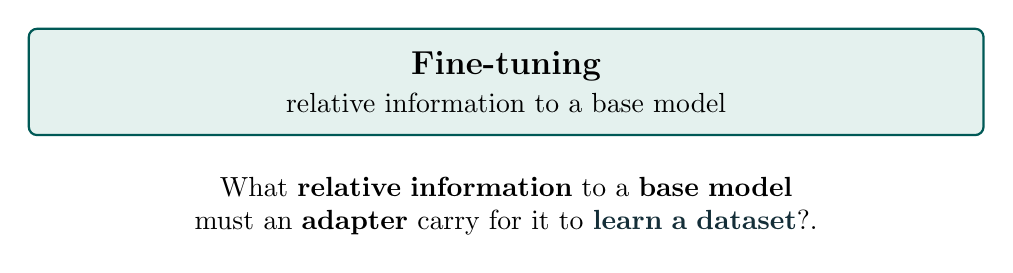
\begin{tikzpicture}
  \node[tealbox,minimum width=\linewidth,minimum height=1.35cm,align=center] (a) {\large\bfseries Fine-tuning\\[2pt]\normalsize relative information to a base model};
  \node[below=0.4cm of a,align=center,text width=.93\linewidth] {What \textbf{relative information} to a \textbf{base model} must an \textbf{adapter} carry for it to \key{\textbf{learn a dataset}}?.};
\end{tikzpicture}
\column{0.48\textwidth}
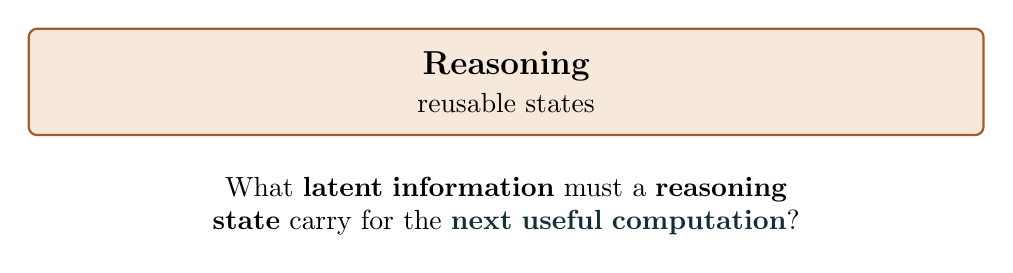
\begin{tikzpicture}
  \node[amberbox,minimum width=\linewidth,minimum height=1.35cm,align=center] (a) {\large\bfseries Reasoning\\[2pt]\normalsize reusable states};
  \node[below=0.4cm of a,align=center,text width=.93\linewidth] {What \textbf{latent information} must a \textbf{reasoning state} carry for the \key{next useful computation}?};
\end{tikzpicture}
\end{columns}
\vfill
\begin{center}
  \tikz\node[fill=Dark,text=white,rounded corners=4pt,inner xsep=12pt,inner ysep=7pt]{\bfseries Relative information = receiver + utility + update rule};
\end{center}
\note{\small\begin{itemize}
  \item « Information » n'est pas une propriété intrinsèque du fichier ou de la trace.
  \item Fine-tuning: le récepteur possède déjà le base model; on mesure le message supplémentaire.
  \item Reasoning: le récepteur doit pouvoir continuer le calcul à partir d'un état.
  \item Les protocoles diffèrent, mais la question conceptuelle est la même.
\end{itemize}}
\end{frame}

% -----------------------------------------------------------------------------
\begin{frame}[plain]
  \begin{tikzpicture}[remember picture,overlay]
    \fill[Dark] (current page.south west) rectangle (current page.north east);
  \end{tikzpicture}
  \vspace{1.0cm}
  {\color{LightTeal}\bfseries PART I}\par\vspace{0.45cm}
  {\color{white}\fontsize{30}{33}\selectfont\bfseries
    Information-theoretic\\
    limits of finetuning in\\[-5pt]
    quantized LLMs\par}
  \vspace{0.55cm}{\color{white!72}\large Quantized models as compressed representations of their training
data}
  \note{\small\begin{itemize}
    \item Point de départ du stage: étudier le fine-tuning sous un angle information-théorique.
    \item Question pratique: après avoir appris un dataset, combien de bits de la mise à jour faut-il réellement conserver?
    \item Le base model est partagé: on ne paie que ce que l'apprentissage ajoute.
  \end{itemize}}
\end{frame}

% -----------------------------------------------------------------------------
\begin{frame}{Abstracting LLMs as autoregressive neural networks}
\framesubtitle{stack of attention/MLP blocks (+ layernorms...) \rightarrow{} a single function $f_{\theta_0}$}
\hspace*{0.06\textwidth}
\begin{columns}[c,onlytextwidth]
\column{0.36\textwidth}
\begin{center}
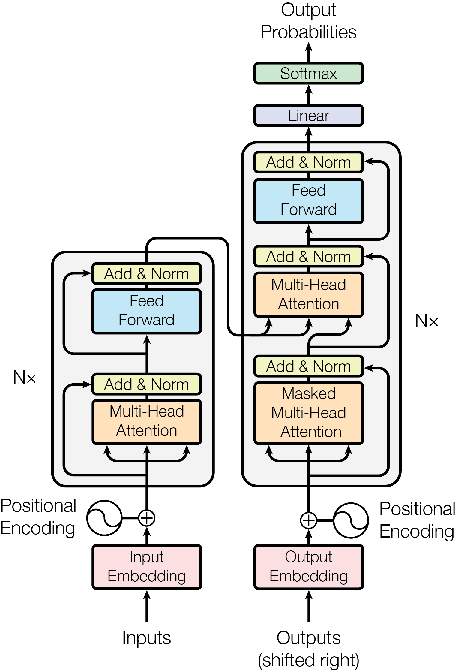
\includegraphics[height=0.58\paperheight]{assets/papers/transformer_vaswani_fig1}
\\[-2pt]
{\scriptsize\color{Muted}\textbf{Source:} Vaswani et al. (2017), Fig.~1}
\end{center}
\column{0.60\textwidth}
\vspace{0.10cm}
\begin{center}
{\color{Teal}\large Autoregressive objective}
\end{center}
\vspace{-0.12cm}
\[
  p_\theta(y_{1:T}\mid x)=\prod_{t=1}^T p_\theta(y_t\mid x,y_{<t})
\]
\vspace{-0.35cm}
\begin{center}\small\color{Muted}prefix $\longrightarrow$ next-token distribution\end{center}
\vspace{0.35cm}
\begin{center}
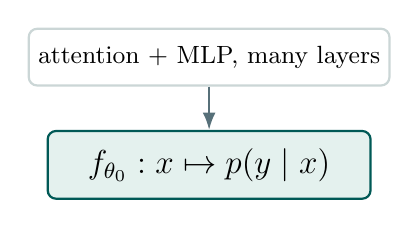
\begin{tikzpicture}
  \node[boxstyle,minimum width=4.1cm,minimum height=.72cm,align=center,font=\small] (m) {attention $+$ MLP, many layers};
  \node[tealbox,below=.55cm of m,minimum width=4.1cm,minimum height=.86cm,align=center] (f) {\large $f_{\theta_0}: x \mapsto p(y\mid x)$};
  \draw[arr] (m)--(f);
\end{tikzpicture}
\end{center}
\end{columns}
\note{\small\begin{itemize}
  \item Voici l'architecture originale du Transformer, telle qu'elle apparaît dans l'article de Vaswani et al.
  \item Le point n'est pas d'en détailler chaque bloc: il s'agit de montrer qu'une LLM est une pile de blocs attention + MLP.
  \item Ce que l'on retient: un préfixe entre, une distribution du prochain token sort.
  \item Pour la Partie I, on peut donc écrire le modèle comme une fonction $f_{\theta_0}$ et étudier la perturbation de paramètres introduite par l'apprentissage.
  \item L'attention et les MLPs restent importants, mais ils n'entrent pas dans la définition de notre mesure.
\end{itemize}}
\end{frame}

% -----------------------------------------------------------------------------
\begin{frame}{Abstracting away the Transformer architecture}
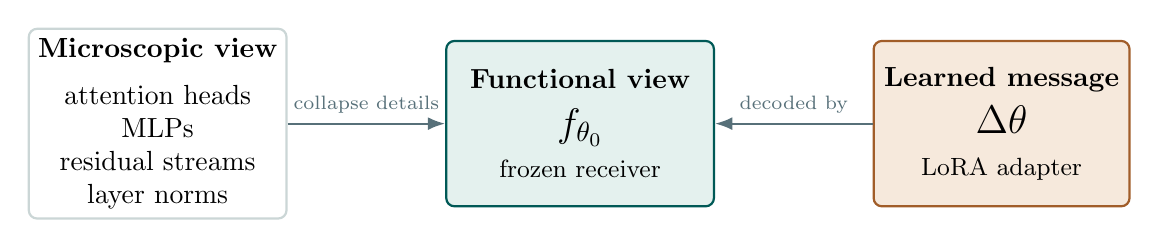
\begin{tikzpicture}[node distance=2.5cm]
  \node[boxstyle,fill=white,minimum width=3.25cm,minimum height=2.1cm,align=center] (micro) {\bfseries Microscopic view\\[5pt] attention heads\\MLPs\\residual streams\\layer norms};
  \node[tealbox,right=2.0cm of micro,minimum width=3.4cm,minimum height=2.1cm,align=center] (coarse) {\bfseries Functional view\\[5pt]\Large $f_{\theta_0}$\\[3pt]\small frozen receiver};
  \node[amberbox,right=2.0cm of coarse,minimum width=3.25cm,minimum height=2.1cm,align=center] (upd) {\bfseries Learned message\\[5pt]\Large $\Delta\theta$\\[3pt]\small LoRA adapter};
  \draw[arr] (micro)-- node[above,align=center,font=\scriptsize,text=Muted]{collapse details} (coarse);
  \draw[arr] (upd)-- node[above,align=center,font=\scriptsize,text=Muted]{decoded by} (coarse);
\end{tikzpicture}
\vspace{0.45cm}
\begin{columns}[T,onlytextwidth]
\column{0.48\textwidth}
\textbf{Definition of rate uses only}
\begin{itemize}\small
  \item fixed $\theta_0$ and adapter layout
  \item serialized update size
  \item held-out behavior after reload
\end{itemize}
\column{0.48\textwidth}
\textbf{Microstructure matters later for}
\begin{itemize}\small
  \item where adapters are inserted
  \item which directions are behaviorally sensitive
  \item predictors of required rate
\end{itemize}
\end{columns}
\vfill
\note{\small\begin{itemize}
  \item Point important à expliciter: on ne prétend pas que l'architecture interne est négligeable en général.
  \item Elle est simplement conditionnée dans notre expérience: même base model, même placement LoRA, même décodeur.
  \item Le rate se définit par la taille du message et le comportement après rechargement; cette définition ne requiert pas de distinguer chaque tête d'attention.
  \item En revanche, la microstructure peut expliquer pourquoi certaines directions coûtent plus cher; c'est justement le rôle des prédicteurs plus tard.
\end{itemize}}
\end{frame}

% -----------------------------------------------------------------------------
\begin{frame}{Fine-tuning = learning a dataset relative to a base model}
\begin{columns}[T,onlytextwidth]
\column{0.56\textwidth}
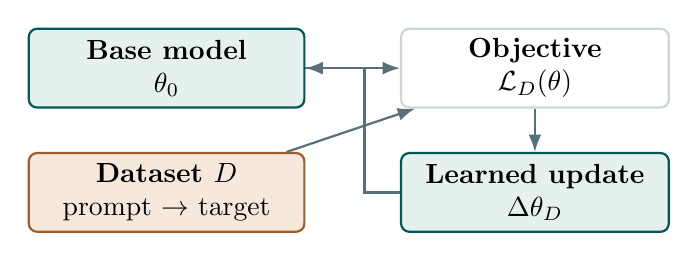
\begin{tikzpicture}[node distance=.45cm]
  \node[tealbox,minimum width=3.5cm,minimum height=1.0cm,align=center] (base) {\bfseries Base model\\$\theta_0$};
  \node[amberbox,below=.55cm of base,minimum width=3.5cm,minimum height=1.0cm,align=center] (data) {\bfseries Dataset $D$\\prompt $\to$ target};
  \node[boxstyle,right=1.2cm of base,minimum width=3.4cm,minimum height=1.0cm,align=center] (obj) {\bfseries Objective\\$\mathcal L_D(\theta)$};
  \node[tealbox,below=.55cm of obj,minimum width=3.4cm,minimum height=1.0cm,align=center] (upd) {\bfseries Learned update\\$\Delta\theta_D$};
  \draw[arr] (base)--(obj); \draw[arr] (data)--(obj); \draw[arr] (obj)--(upd);
  \draw[arr] (upd.west) -- ++(-.45,0) |- (base.east);
\end{tikzpicture}
\column{0.40\textwidth}
\small
\begin{block}{Full fine-tuning}
$\theta_D=\theta_0+\Delta\theta_D$\\Most parameters may move.
\end{block}
\begin{block}{Parameter-efficient fine-tuning}
Keep $\theta_0$ fixed; learn a much smaller task-specific object.\tinycite{aghajanyan2021intrinsic}
\end{block}
\end{columns}
\vfill
\begin{center}\begin{minipage}{0.86\textwidth}\centering\bfseries The relative information of a dataset to a base model needs to be carried by the update (here, the adapter).\end{minipage}\end{center}
\note{\small\begin{itemize}
  \item « Learning a dataset »: l'optimisation pousse le base model à corriger certaines prédictions sur les exemples du corpus.
  \item Ce qui est appris dépend donc déjà de $\theta_0$.
  \item Les résultats d'intrinsic dimension motivent l'idée qu'une adaptation utile peut vivre dans un espace beaucoup plus petit que tous les paramètres.
  \item Notre objet d'étude devient la description de $\Delta\theta_D$ conditionnellement au base model.
\end{itemize}}
\end{frame}

% -----------------------------------------------------------------------------
\begin{frame}{Parameter-efficient finetuning with LoRA}
\begin{columns}[c,onlytextwidth]
\column{0.46\textwidth}
\begin{center}

\includegraphics[height=0.50\paperheight]{assets/papers/lora_hu_fig1}
\end{center}
\column{0.50\textwidth}
\[
W' = W + \Delta W,\qquad
\Delta W=\frac{\alpha}{r}BA
\]
\vspace{-0.15cm}
\begin{itemize}\small\setlength\itemsep{2.5pt}
  \item $W$ is \key{frozen} and already shared
  \item only $A,B$ are trained, with $r\ll d$
  \item $r(d_{in}+d_{out})$ values instead of $d_{in}d_{out}$
\end{itemize}
\vspace{0.20cm}
\begin{center}
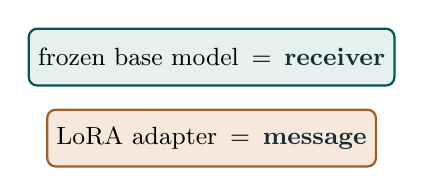
\begin{tikzpicture}[node distance=.3cm]
  \node[tealbox,minimum width=3.5cm,minimum height=.72cm,align=center,font=\small] (r) {frozen base model \,=\, \key{receiver}};
  \node[amberbox,below=.28cm of r,minimum width=3.5cm,minimum height=.72cm,align=center,font=\small] (m) {LoRA adapter \,=\, \key{message}};
\end{tikzpicture}
\end{center}
\end{columns}
\vspace{0.10cm}

\figsource{hu2022lora}{Fig.~1}
\note{\small\begin{itemize}
  \item Figure originale de Hu et al.: $W$ reste gelée, on n'apprend que $A$ et $B$.
  \item $BA$ est de rang faible, avec $r$ très petit devant $d$.
  \item Cela fournit un petit objet appris, séparé du base model.
  \item C'est précisément ce qui rend possible notre lecture « message + receiver »: le base model est déjà partagé, on ne transmet que l'adapter.
  \item Mais attention: le rang ne donne pas un nombre de bits: les valeurs numériques doivent encore être représentées.
  \item Première distinction scientifique de la Partie I: dimension paramétrique et information utile ne sont pas la même chose.
\end{itemize}}
\end{frame}

% -----------------------------------------------------------------------------
\begin{frame}{QLoRA: even more parameter efficient finetuning}
\begin{center}
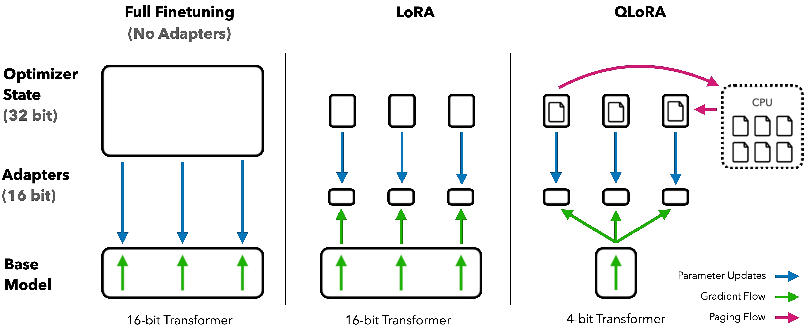
\includegraphics[width=0.710\textwidth]{assets/papers/qlora_detmers_fig1}
\end{center}
\vspace{0.10cm}
\begin{columns}[T,onlytextwidth]
\column{0.48\textwidth}
\textbf{QLoRA quantization}
\begin{itemize}\small\setlength\itemsep{1.5pt}
  \item the \key{frozen base model} (NF4, 4-bit)
  \item adapters remain trainable in 16-bit
\end{itemize}
\column{0.48\textwidth}
\textbf{We then:}
\begin{itemize}\small\setlength\itemsep{1.5pt}
  \item fix one trained adapter
  \item compress \key{the learned update itself}
\end{itemize}
\end{columns}
\vspace{0.18cm}
\figsource{dettmers2023qlora}{Fig.~1}
\note{\small\begin{itemize}
  \item Figure originale de Dettmers et al.: trois régimes, full finetuning, LoRA, QLoRA.
  \item Distinction essentielle: QLoRA quantifie le \emph{backbone} gelé, pas l'adapter. Les paramètres LoRA restent entraînables en précision plus élevée.
  \item C'est donc d'abord une technique d'efficacité mémoire à l'entraînement.
  \item Notre travail pose ensuite une autre question: combien peut-on compresser l'update appris tout en conservant son comportement?
  \item Les deux parlent de quantification, mais l'objet quantifié n'est pas le même.
\end{itemize}}
\end{frame}

% -----------------------------------------------------------------------------
\begin{frame}{Some information theory: Rate--distortion}
\begin{center}
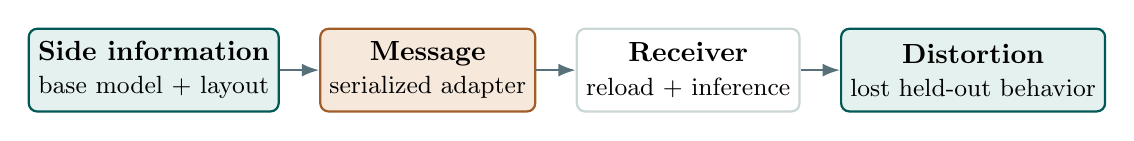
\begin{tikzpicture}[node distance=.45cm]
  \node[tealbox,minimum width=2.55cm,minimum height=1.05cm,align=center] (side) {\bfseries Side information\\\small base model + layout};
  \node[amberbox,right=.5cm of side,minimum width=2.45cm,minimum height=1.05cm,align=center] (msg) {\bfseries Message\\\small serialized adapter};
  \node[boxstyle,right=.5cm of msg,minimum width=2.6cm,minimum height=1.05cm,align=center] (recv) {\bfseries Receiver\\\small reload + inference};
  \node[tealbox,right=.5cm of recv,minimum width=2.85cm,minimum height=1.05cm,align=center] (u) {\bfseries Distortion\\\small lost held-out behavior};
  \draw[arr] (side)--(msg); \draw[arr] (msg)--(recv); \draw[arr] (recv)--(u);
\end{tikzpicture}
\end{center}
\vspace{0.35cm}
\begin{columns}[T,onlytextwidth]
\column{0.46\textwidth}
\centering\footnotesize
\phantom{Here:}
\[
\begin{aligned}
R^*(D)&=\min R\\[-2pt]
&\text{s.t.}\quad d(\hat\theta,\theta)\le D
\end{aligned}
\]
\column{0.46\textwidth}
\centering\footnotesize
Here:
\[
\begin{aligned}
R^*(0.90)&=\min\{R:\\[-2pt]
&\mathrm{Retain}(R)\ge .90\}.
\end{aligned}
\]
\end{columns}
\vfill
\begin{center}\bfseries Rate is defined purely relatively to a receiver and a distortion/utility.\end{center}
\tinycite{berger1971rate,cover2006elements,grunwald2019mdl}
\note{\small\begin{itemize}
  \item Rate--distortion pose exactement la bonne forme de question: le message le plus court sous une contrainte d'erreur.
  \item Mais il faut définir l'erreur au niveau du comportement du récepteur, pas seulement dans l'espace des poids.
  \item Le base model, le layout LoRA et le décodeur sont de la side information partagée.
  \item $R^*$ reste un minimum empirique sur la ladder de codecs testée, pas une borne universelle de Shannon.
\end{itemize}}
\end{frame}

\begin{frame}{Can LoRA rank stand in for a rate?}
\framesubtitle{First hypothesis}
\begin{columns}[T,onlytextwidth]
\column{0.46\textwidth}
\begin{block}{Question}
If useful adaptation lives in a small subspace (c.f. LoRA's rank), does the smallest effective rank behave like an information budget? \\
\vspace{0.25cm}
Rank directly limits how many degrees of freedom the update may use. If rank is equivalent to the budget, the held-out gain should saturate exactly where the budget is exhausted.
\end{block}
\column{0.46\textwidth}
\small
\textbf{Setup}
\begin{itemize}\setlength\itemsep{5pt}
  \item Qwen2.5-0.5B, QLoRA sweep
  \item ranks $\in\{0,2,4,8,16\}$; rank 0 = frozen baseline
  \item instruction data from Alpaca and Dolly
  \item dataset variants: duplicated examples, more regular templates
\end{itemize}
\vspace{0.3cm}
\chip{prediction} gain saturates at the smallest sufficient rank
\end{columns}
\note{\small\begin{itemize}
  \item Première hypothèse: le rang LoRA comme proxy bon marché de ce qu'un finetuning écrit.
  \item Design minimal: un seul bouton, le rang, et on regarde où le gain sature.
  \item Variantes de dataset: duplication d'exemples et templates plus réguliers.
\end{itemize}}
\end{frame}
% -----------------------------------------------------------------------------
% -----------------------------------------------------------------------------
\begin{frame}{Can LoRA rank stand in for a rate? Not quite.}
\begin{columns}[c,onlytextwidth]
\column{0.52\textwidth}
\centering
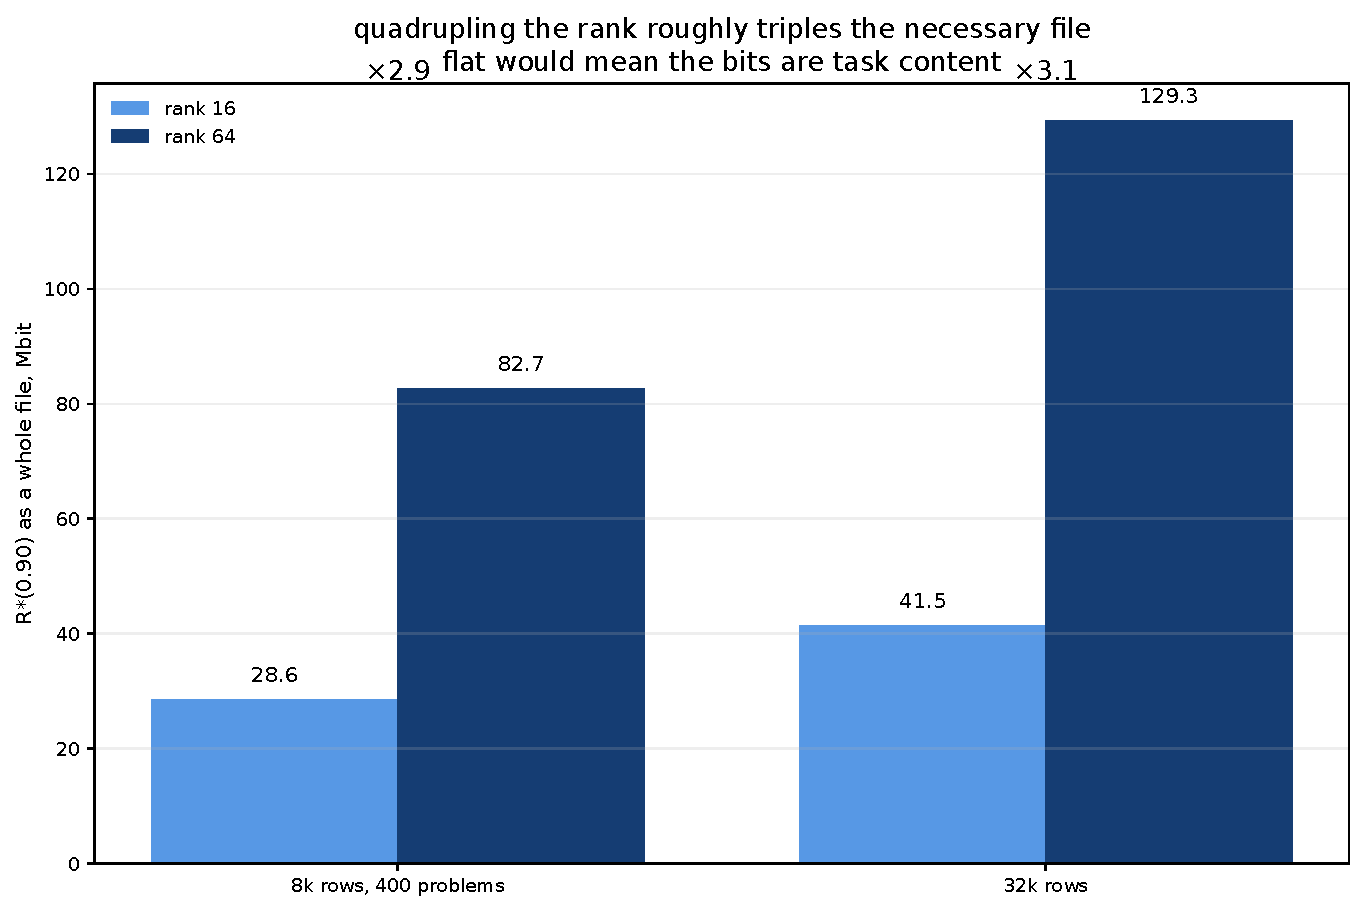
\includegraphics[width=\linewidth,trim=0bp 0bp 0bp 39bp,clip]{assets/real/rank_scaling.pdf}
\par\vspace{0.1cm}
{\footnotesize\color{Muted} smallest file retaining 90\% of the gain, Mbit\par}
\column{0.44\textwidth}
\par Instead of a rough match in compressed adapter size, quadrupling the rank instead roughly triples it: {\color{Teal}\bfseries $\times2.9$}, {\color{Teal}\bfseries $\times3.1$}.
\vspace{0.35cm}
\par Our other pilot knobs failed too: duplication changes optimization exposure, surface compressibility is not a clean intervention.
\end{columns}
\vspace{0.25cm}
\begin{center}\begin{minipage}{0.88\textwidth}\centering\bfseries\small
Next question: hold one learned update fixed, and vary only how many bits are used to store it.
\end{minipage}\end{center}
\note{\small\begin{itemize}
  \item Chaque paire de barres: même corpus, même comportement à préserver, seul le rang change.
  \item Si le fichier mesurait le contenu de la tâche, les deux barres seraient à la même hauteur.
  \item Or quadrupler le rang triple à peu près le fichier: facteurs 2.9 et 3.1.
  \item Le rang dimensionne le contenant, pas le contenu: il compte des degrés de liberté.
  \item Les autres leviers pilotes échouent aussi: duplication et compressibilité de surface ne sont pas des interventions propres.
  \item D'où le protocole suivant: figer une mise à jour apprise et ne faire varier que son code.
\end{itemize}}
\end{frame}
% -----------------------------------------------------------------------------
% -----------------------------------------------------------------------------
\begin{frame}{Exact-rate protocol: one update, many codes}
\begin{columns}[c,onlytextwidth]
\column{0.48\textwidth}
\begin{center}
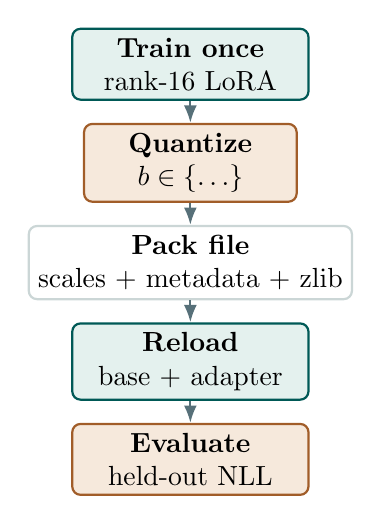
\begin{tikzpicture}[node distance=.28cm]
  \node[tealbox,minimum width=3.0cm,minimum height=.82cm,align=center] (train) {\bfseries Train once\\rank-16 LoRA};
  \node[amberbox,below=of train,minimum width=2.7cm,minimum height=.82cm,align=center] (q) {\bfseries Quantize\\$b\in\{\ldots\}$};
  \node[boxstyle,below=of q,minimum width=3.5cm,minimum height=.82cm,align=center] (pack) {\bfseries Pack file\\scales + metadata + zlib};
  \node[tealbox,below=of pack,minimum width=3.0cm,minimum height=.82cm,align=center] (load) {\bfseries Reload\\base + adapter};
  \node[amberbox,below=of load,minimum width=3.0cm,minimum height=.82cm,align=center] (eval) {\bfseries Evaluate\\held-out NLL};
  \draw[arr] (train)--(q);\draw[arr] (q)--(pack);\draw[arr] (pack)--(load);\draw[arr] (load)--(eval);
\end{tikzpicture}
\end{center}
\column{0.48\textwidth}
\begin{center}
\[
R=\frac{8\times\text{file bytes}}{P}
\]
\small $P=$ number of values in the original adapter
\vspace{0.35cm}
\[
\mathrm{Retain}(R)=\frac{L_0-L_R}{L_0-L_{raw}}
\]
\small $L_0$: frozen base; $L_{raw}$: uncompressed adapter
\end{center}
\end{columns}
\note{\small\begin{itemize}
  \item On entraîne un adapter une seule fois et on fige le checkpoint.
  \item Chaque point de courbe = autre représentation numérique du même update.
  \item Le taux vient de la vraie taille de fichier, métadonnées incluses, normalisée par le nombre de valeurs originales.
  \item Retention = fraction du gain sur le base model qui survit.
\end{itemize}}
\end{frame}

\begin{frame}{Experiment: can a fixed budget be allocated more intelligently?}
\begin{columns}[T,onlytextwidth]
\column{0.46\textwidth}
\begin{block}{Question}
At a matched file size, does spending bits where reconstruction is hardest preserve more behavior than uniform precision?
\end{block}
\vspace{0.25cm}
\begin{block}{Why this design answers it}
\small The adapter checkpoint is fixed, so the two codecs differ only in allocation. Any difference in retained gain is attributable to where the bits went.
\end{block}
\column{0.46\textwidth}
\small
\textbf{Setup}
\begin{itemize}\setlength\itemsep{5pt}
  \item one rank-16 LoRA on 32k MetaMathQA rows, Mistral-7B on an NF4 base
  \item per row of a LoRA factor: drop, or encode at 1, 2, 3, 4, 8 bits
  \item Lagrangian objective trades reconstruction error against code length
  \item control: plain zero-free uniform code at the same rate
\end{itemize}
\vspace{0.25cm}
\chip{prediction} error-aware allocation wins at equal rate
\note{\small\begin{itemize}
  \item Le budget est fixé: seule l'allocation change entre les deux codecs.
  \item L'allocateur peut supprimer une ligne ou la coder sur 1, 2, 3, 4 ou 8 bits.
  \item Hypothèse: les lignes les plus dures à reconstruire sont celles qui comptent pour le comportement.
\end{itemize}}
\end{columns}
\end{frame}
% -----------------------------------------------------------------------------
% -----------------------------------------------------------------------------
\begin{frame}{Weight reconstruction error is not behavioral distortion}
\framesubtitle{A negative result that forces output-level evaluation}
\begin{center}
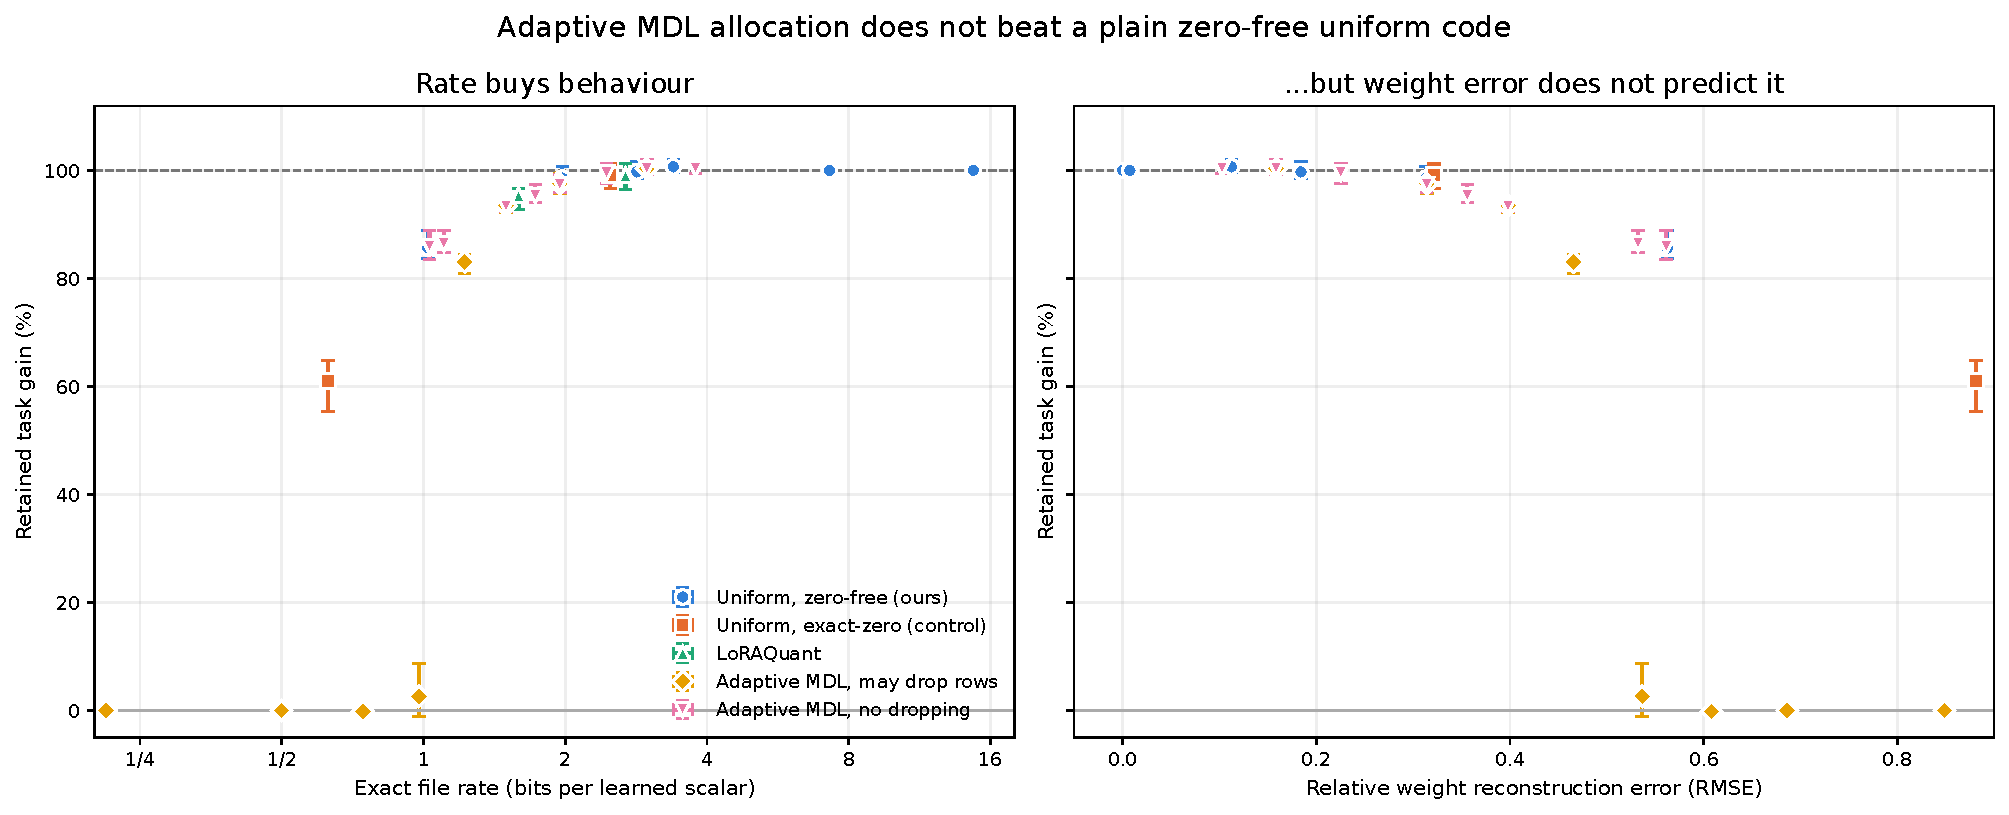
\includegraphics[width=0.95\textwidth,trim=0bp 0bp 0bp 26bp,clip]{assets/real/mdl_vs_uniform.pdf}
\end{center}
\vspace{0.05cm}
{\centering\small
{\bfseries\color{Teal}85.7\%} retained gain, uniform code \; · \;
{\bfseries\color{Teal}2.6\%} retained gain, adaptive RMSE\par}
\vspace{0.15cm}
\note{\small\begin{itemize}
  \item Premier allocateur adaptatif: minimiser une erreur de reconstruction des facteurs LoRA sous budget.
  \item Contre-exemple: RMSE similaire, mais environ 85.7\% de gain conservé pour le sign code uniforme contre 2.6\% pour l'adaptatif.
  \item Conclusion: la norme dans l'espace des poids n'est pas une distortion suffisante.
  \item Il faut mesurer directement le comportement après rechargement.
\end{itemize}}
\end{frame}

\begin{frame}{How do we interpret this negative result?}
\begin{columns}[T,onlytextwidth]
\column{0.48\textwidth}
\begin{block}{Ruled out}
\small Global weight error is not a sufficient measure of useful adapter information: two reconstructions with similar RMSE can preserve very different behavior.
\end{block}
\column{0.48\textwidth}
\begin{block}{Implication}
\small The distortion must be read at the receiver's output, which is exactly the $\mathrm{Retain}(R)$ criterion the protocol already uses.
\end{block}
\end{columns}
\vfill
\begin{center}\begin{minipage}{0.88\textwidth}\centering\bfseries
The question shifts from \emph{where} to spend a fixed budget to what determines how large the required budget is.
\end{minipage}\end{center}
\note{\small\begin{itemize}
  \item Conclusion scientifique: la norme dans l'espace des poids ne suffit pas comme distortion.
  \item La mesure doit se faire à la sortie du receveur, pas sur les poids.
  \item Et la question change: non plus où dépenser les bits, mais ce qui fixe leur nombre.
\end{itemize}}
\end{frame}
% -----------------------------------------------------------------------------
\begin{frame}{Experiment: does more distinct data cost more bits?}
\framesubtitle{Compute-matched distinct-example panel}
\begin{columns}[T,onlytextwidth]
\column{0.46\textwidth}
\begin{block}{Question}
Does the required rate grow with the amount of distinct training data, at fixed training exposure?
\end{block}
\vspace{0.25cm}
\begin{block}{Why this design answers it}
\small Holding both optimizer steps and total presentations fixed removes the pilot confound: only the number of distinct rows changes.
\end{block}
\column{0.46\textwidth}
\small
\textbf{Setup}
\begin{itemize}\setlength\itemsep{5pt}
  \item MetaMathQA, 2{,}000 to 32{,}000 distinct examples
  \item optimizer steps fixed at 2{,}000
  \item total example presentations fixed at 32{,}000
  \item 15 runs, same codec ladder, $R^*(0.90)$ read off each curve
\end{itemize}
\vspace{0.25cm}
\chip{prediction} $R^*$ increases with distinct rows
\end{columns}
\note{\small\begin{itemize}
  \item On fait varier le nombre d'exemples distincts sans changer l'exposition d'optimisation.
  \item Steps et présentations totales sont fixés: c'est ce qui rend l'intervention propre.
  \item On lit ensuite R*(0.90) sur chaque courbe de rétention.
\end{itemize}}
\end{frame}
% -----------------------------------------------------------------------------
% -----------------------------------------------------------------------------
\begin{frame}{More distinct content generally requires more adapter rate}
\framesubtitle{Compute-matched MetaMathQA pilot: 15 runs}
\begin{columns}[T,onlytextwidth]
\column{0.62\textwidth}
\vspace{0.15cm}
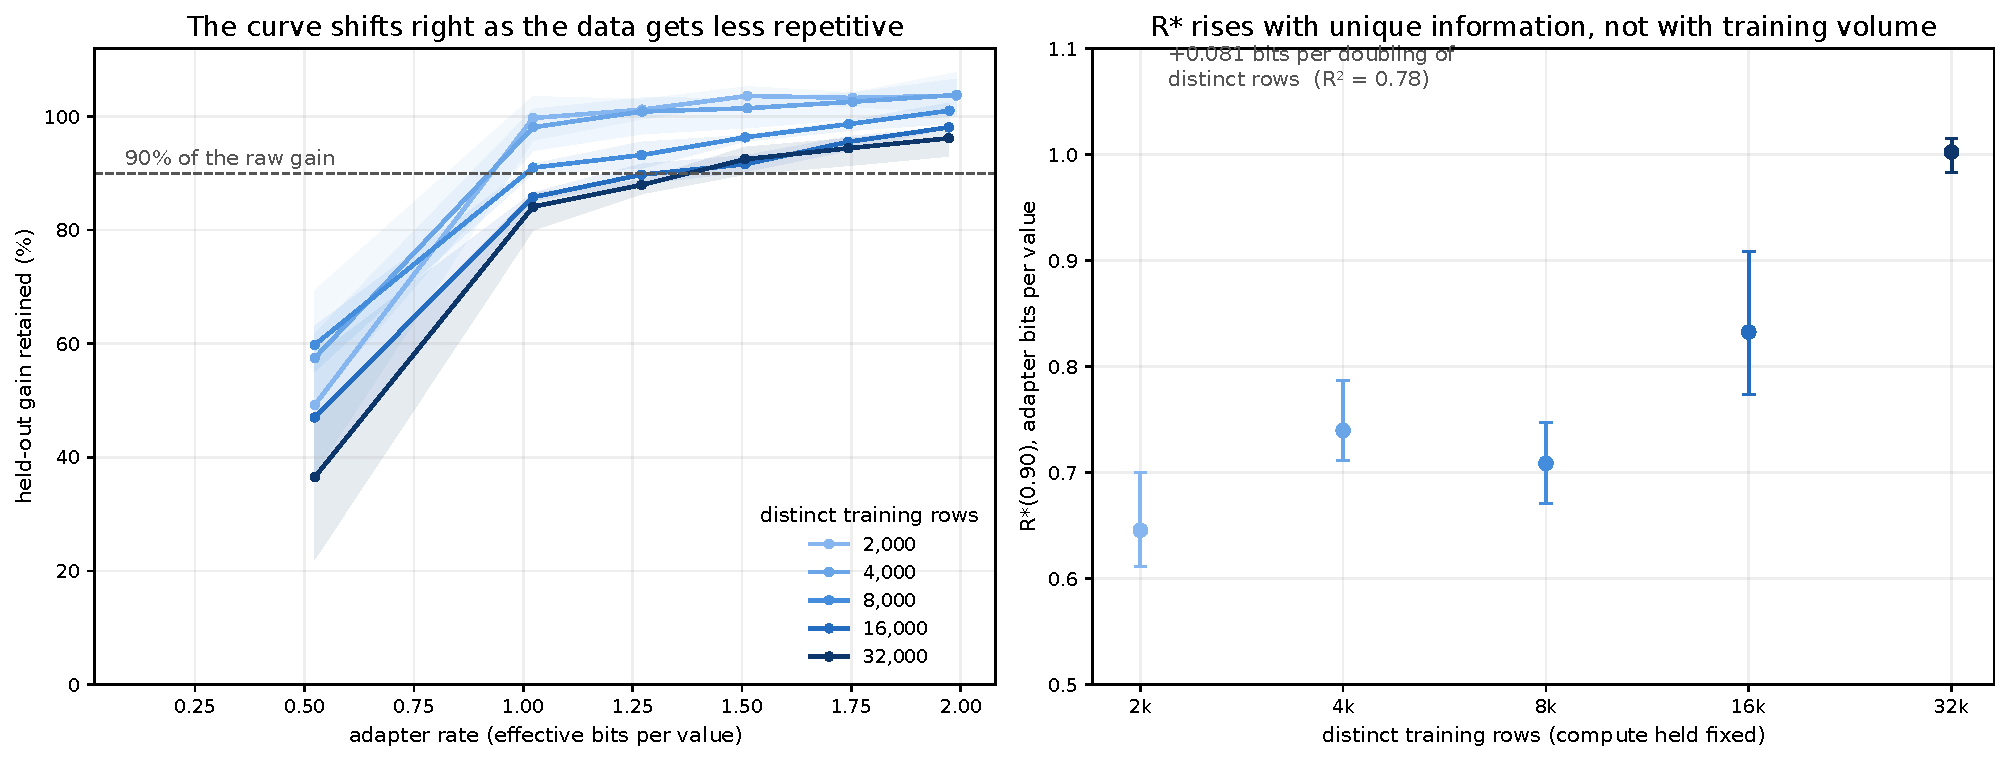
\includegraphics[width=\linewidth,trim=487bp 0bp 0bp 44bp,clip]{assets/real/rate_vs_retention.pdf}
\column{0.34\textwidth}
\vspace{0.4cm}
\stat{$R^2=0.78$}{internal fit}
\vspace{0.55cm}
\small
\begin{itemize}
  \item optimizer steps fixed
  \item total presentations fixed
  \item trend not perfectly monotone
  \item content-diversity control: $0.682\to0.742$
\end{itemize}
\end{columns}
\note{\small\begin{itemize}
  \item Ici on fixe 2 000 optimizer steps et 32 000 présentations, puis on varie seulement le nombre d'exemples distincts.
  \item Le taux requis augmente globalement; fit interne $R^2=0.78$.
  \item Ce n'est pas encore une loi universelle: le trend n'est pas parfaitement monotone.
  \item Un contrôle séparé de diversité de contenu donne la même direction, de 0.682 à 0.742 bits/value.
\end{itemize}}
\end{frame}

\begin{frame}{Distinct rows or distinct content?}
\framesubtitle{Two controls behind the same trend}
\begin{center}
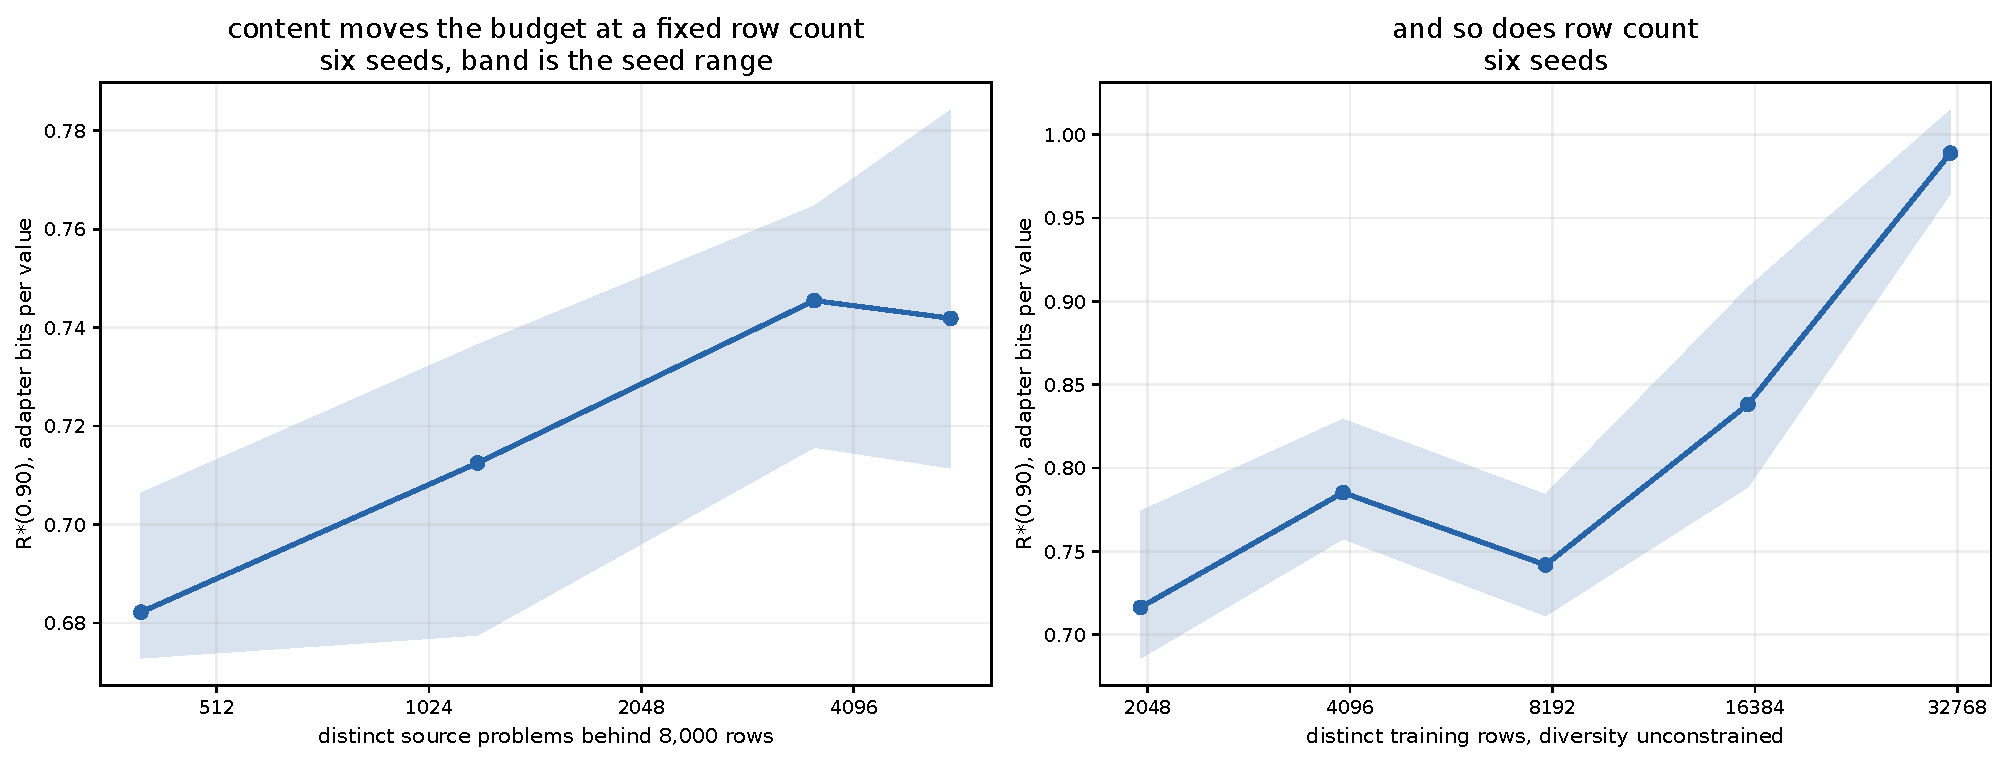
\includegraphics[width=0.76\textwidth,trim=0bp 0bp 0bp 8bp,clip]{assets/real/content_and_rows.pdf}
\end{center}
\vspace{0.1cm}
{\centering\small
left: {\bfseries\color{Teal}$0.682\to0.742$} bits per value as source problems grow behind a fixed 8{,}000-row corpus \; · \;
right: row count moves the budget too, six seeds\par}
\vspace{0.15cm}
\begin{center}\begin{minipage}{0.9\textwidth}\centering\bfseries
Content diversity, not just row count, moves the required rate --- but more diverse data also improved the model more.
\end{minipage}\end{center}
\note{\small\begin{itemize}
  \item Contrôle gauche: 8 000 exemples fixes, on fait varier le nombre de problèmes sources.
  \item R* moyen passe de 0.682 à 0.742 bits par valeur sur six graines.
  \item Contrôle droit: le nombre de lignes distinctes bouge aussi le budget à exposition fixée.
  \item Objection restante: les adapters les plus divers améliorent aussi plus le modèle.
\end{itemize}}
\end{frame}
% -----------------------------------------------------------------------------
\begin{frame}{Is the rate just a function of how much was learned?}
\framesubtitle{Two controls that vary learned gain on purpose}
\begin{columns}[T,onlytextwidth]
\column{0.50\textwidth}
\begin{block}{Style rewrites}
\small Same answers rewritten in five deterministic styles, from short plain responses to symbolic ones.
\end{block}
\vspace{0.2cm}
\small
learned gain \quad {\color{Teal}\bfseries $0.555\to1.062$} bits/token\par
\vspace{2pt}
required rate \quad {\color{Teal}\bfseries $0.684\to0.763$} bits/value
\column{0.44\textwidth}
\begin{block}{Optimizer-budget sweep}
\small A separate 16-fold sweep changes how much is learned while the data content stays fixed.
\end{block}
\vspace{0.2cm}
\small Again no matching rate increase.
\vspace{0.35cm}
\par\small Earlier math runs had suggested the opposite: over 48 rank-16 runs, held-out gain explained 56\% of the variance in $R^*$ --- but over a narrow range of gains.
\end{columns}
\vfill
\begin{center}\begin{minipage}{0.9\textwidth}\centering\bfseries
Nearly doubling the learned behavior barely moves the required rate: improvement alone does not determine it.
\end{minipage}\end{center}
\note{\small\begin{itemize}
  \item Deux façons différentes de faire varier le gain appris, à contenu constant.
  \item Les réécritures de style doublent presque le gain, mais R* bouge à peine.
  \item Le sweep d'optimisation ne produit pas non plus l'augmentation attendue.
  \item Ensemble, ils éliminent le gain comportemental seul comme déterminant du taux.
\end{itemize}}
\end{frame}
% -----------------------------------------------------------------------------
\begin{frame}{Control: a task whose source information we know by construction}
\framesubtitle{An uncalibrated proxy is ruled out --- but source bits still do not explain adapter rate}
\begin{columns}[T,onlytextwidth]
\column{0.42\textwidth}
\begin{block}{Question}
\small Is our information proxy calibrated at all, when the true number of source bits is known?
\end{block}
\vspace{0.15cm}
\small
\textbf{Setup}
\begin{itemize}\setlength\itemsep{3pt}
  \item each prompt maps to one of 16 one-token labels
  \item conditions differ in the number of independent 4-bit assignments
  \item description length estimated with a conditional prequential code
\end{itemize}
\column{0.54\textwidth}
\centering
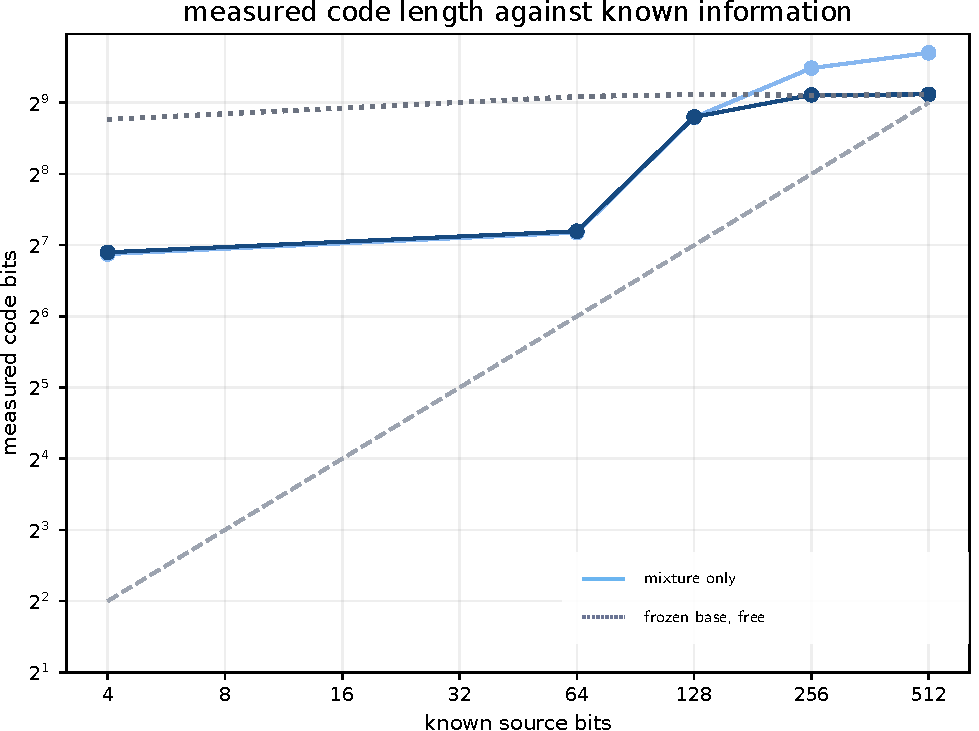
\includegraphics[width=0.86\linewidth]{assets/real/known_information_validation.pdf}
\par\vspace{0.1cm}
{\footnotesize the code orders the 4-, 64-, 128-, 256- and 512-bit conditions correctly, within $1.1$--$3.5\times$ the known source count\par}
\end{columns}
\note{\small\begin{itemize}
  \item Tâche synthétique: on construit nous-mêmes le nombre de bits sources.
  \item Le code prequential conditionnel retrouve le bon ordre des conditions.
  \item Il reste dans un facteur 1.1 à 3.5 du compte connu: le proxy n'est pas absurde.
  \item Mais cela n'explique toujours pas le taux d'adapter.
\end{itemize}}
\end{frame}
% -----------------------------------------------------------------------------
\begin{frame}{Experiment: does a dataset have one intrinsic adapter cost?}
\framesubtitle{Change the receiver, keep everything else fixed}
\begin{columns}[T,onlytextwidth]
\column{0.46\textwidth}
\begin{block}{Question}
If cost were a property of the corpus, its ordering across corpora should survive a change of frozen model.
\end{block}
\vspace{0.25cm}
\begin{block}{Why this design answers it}
\small Changing the frozen model is a direct change of receiver, with the dataset, rank, epochs and codec held fixed. A reversal in ordering falsifies intrinsic cost outright.
\end{block}
\column{0.46\textwidth}
\small
\textbf{Setup}
\begin{itemize}\setlength\itemsep{5pt}
  \item five corpora: instruction, summarization, math, code, dialogue
  \item two frozen receivers: Mistral-7B and Qwen2.5-7B
  \item same LoRA rank, example count, epochs and codec
  \item 3 independently trained adapters per cell, 30 rate curves
\end{itemize}
\vspace{0.25cm}
\chip{prediction} ordering is preserved if cost is intrinsic
\end{columns}
\note{\small\begin{itemize}
  \item Test direct de la dépendance au receveur: on ne change que le modèle gelé.
  \item Cinq corpus, deux modèles, tout le reste identique, trois graines par cellule.
  \item Si le coût était intrinsèque au dataset, l'ordre des corpus devrait être conservé.
\end{itemize}}
\end{frame}
% -----------------------------------------------------------------------------
% -----------------------------------------------------------------------------
\begin{frame}{The same dataset has a different cost for a different base model}
\framesubtitle{$R^*(0.90)$ in bits per original adapter value; 3 seeds per cell}
\begin{columns}[T,onlytextwidth]
\column{0.67\textwidth}
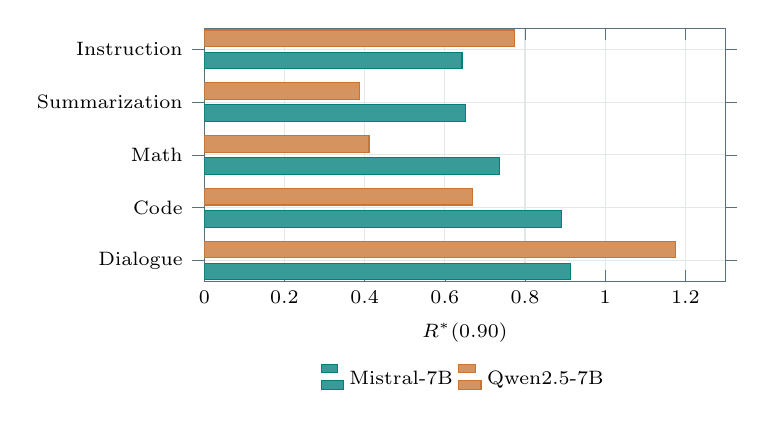
\begin{tikzpicture}
\begin{axis}[
  xbar,bar width=6pt,width=8.2cm,height=4.8cm,
  symbolic y coords={Dialogue,Code,Math,Summarization,Instruction},ytick=data,
  xmin=0,xmax=1.3,
  axis line style={draw=Muted},tick style={draw=Muted},
  ticklabel style={font=\scriptsize},label style={font=\scriptsize},
  xlabel={$R^*(0.90)$},
  legend style={font=\scriptsize,draw=none,at={(.5,-.30)},anchor=north,legend columns=2},
  grid=major,grid style={Line!55}]
  \addplot[fill=Teal!78,draw=Teal] coordinates{(.913,Dialogue)(.891,Code)(.737,Math)(.652,Summarization)(.643,Instruction)};
  \addplot[fill=Amber!78,draw=Amber] coordinates{(1.176,Dialogue)(.668,Code)(.411,Math)(.388,Summarization)(.774,Instruction)};
  \legend{Mistral-7B,Qwen2.5-7B}
\end{axis}
\end{tikzpicture}
\column{0.29\textwidth}
\vspace{0.45cm}
\small
\textbf{Ordering reverses.}
\vspace{0.25cm}
\begin{itemize}\setlength\itemsep{7pt}
  \item summarization: $0.652\to0.388$
  \item instruction: $0.643\to0.774$
  \item dialogue remains expensive
\end{itemize}
\end{columns}
\vfill
\begin{center}\bfseries Dataset ``information'' is relative to the model that must absorb it.\end{center}
\note{\small\begin{itemize}
  \item Test direct du caractère relatif au récepteur: mêmes cinq corpus, même protocole, deux base models.
  \item L'ordre des coûts change fortement entre Mistral et Qwen.
  \item Donc un dataset n'impose pas un coût d'adapter intrinsèque.
  \item Cette expérience motive de regarder ce que le dataset demande spécifiquement à chaque modèle de corriger.
\end{itemize}}
\end{frame}

\begin{frame}{Replicating the diversity effect on two structured tasks}
\framesubtitle{Fixed example count; only the number of domains or companies changes}
\begin{center}
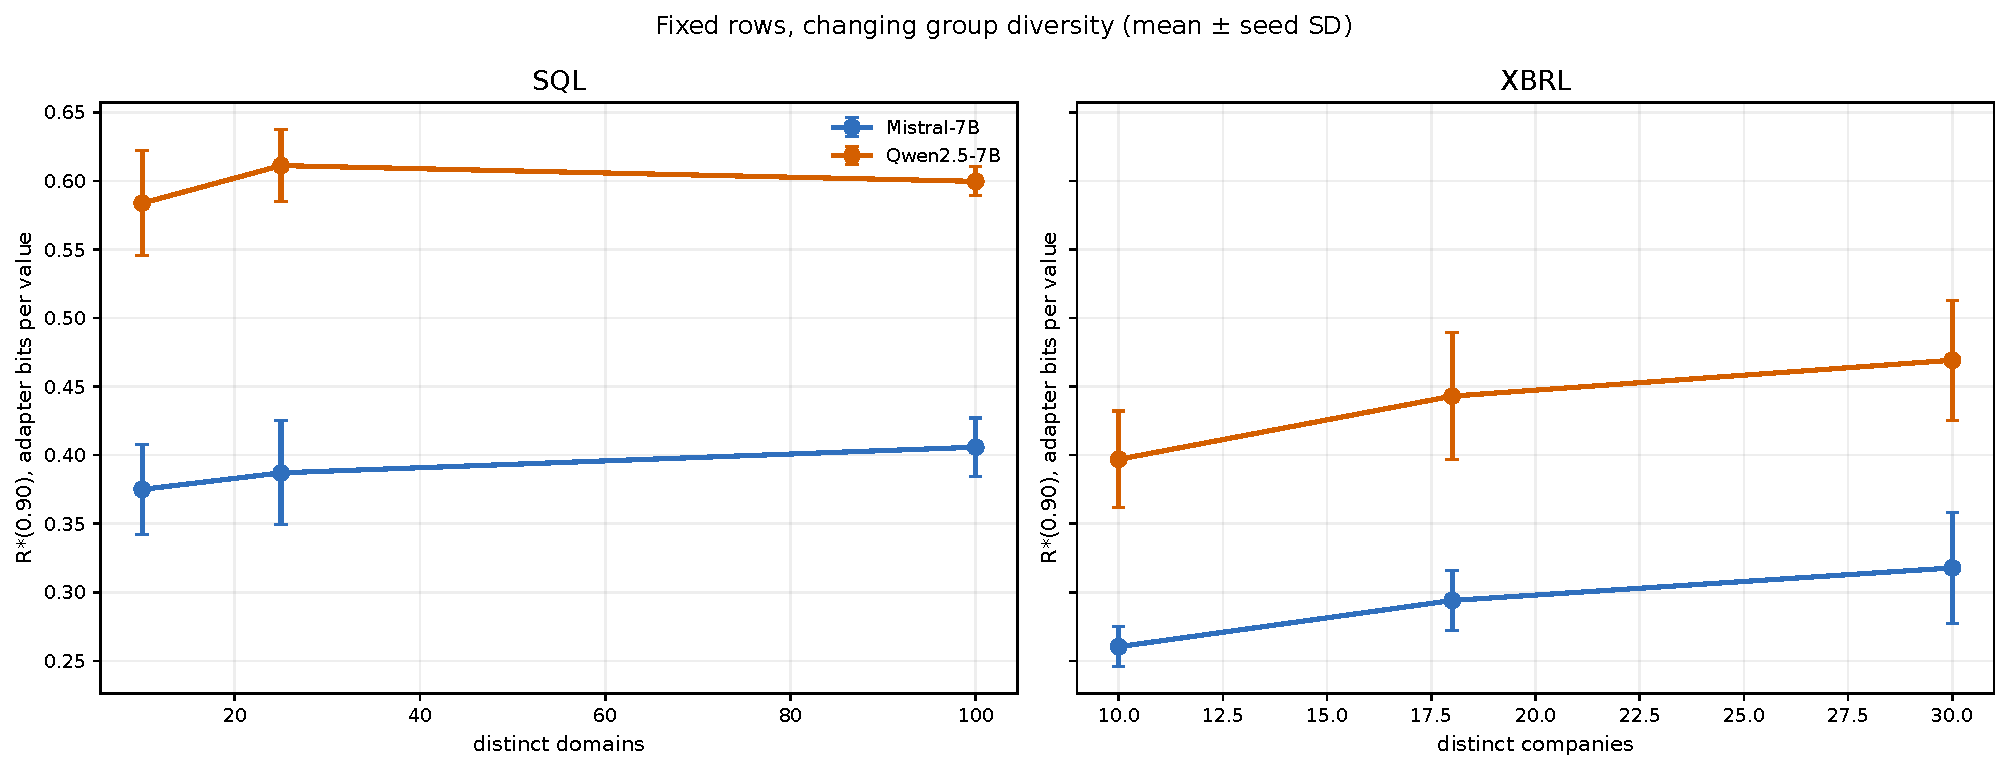
\includegraphics[width=0.84\textwidth,trim=0bp 0bp 0bp 10bp,clip]{assets/real/diversity_replication.pdf}
\end{center}
\vspace{0.1cm}
\begin{columns}[T,onlytextwidth]
\column{0.46\textwidth}
\small XBRL moves in the same direction in all six matched model--seed comparisons.
\column{0.46\textwidth}
\small SQL changes much less, and inconsistently across seeds.
\end{columns}
\vspace{0.15cm}
\begin{center}\begin{minipage}{0.9\textwidth}\centering\bfseries
Content diversity matters in some tasks and not others --- so it is not the underlying quantity either.
\end{minipage}\end{center}
\note{\small\begin{itemize}
  \item On garde le nombre d'exemples fixe et on fait varier le nombre de domaines ou d'entreprises.
  \item XBRL: même direction dans les six comparaisons appariées modèle-graine.
  \item SQL: effet faible et instable selon les graines.
  \item L'intervention XBRL n'est pas parfaitement propre: la couverture du support change aussi.
\end{itemize}}
\end{frame}
% -----------------------------------------------------------------------------
\begin{frame}{Experiment: what does the dataset ask \emph{this} model to correct?}
\framesubtitle{A model-relative candidate, screened against ten alternatives}
\begin{columns}[T,onlytextwidth]
\column{0.48\textwidth}
\begin{block}{Question}
Can a quantity computed on the frozen model, before training, order the required adapter rate?
\end{block}
\vspace{0.2cm}
\small
For a scored token the output-head gradient factorizes as $g_{it}=h_{it}\otimes(p_{it}-e_{y_{it}})$: what the model is representing, times how its prediction must change.
\column{0.46\textwidth}
\small
\textbf{Screen}
\begin{itemize}\setlength\itemsep{5pt}
  \item 22 distinct model--dataset conditions, 7 task families, 2 frozen 7B receivers
  \item ranked by within-model $\rho$ and by RMSE on a held-out task family
  \item permutation test corrected for screening ten candidate measures
\end{itemize}
\end{columns}
\vfill
\begin{center}\begin{minipage}{0.9\textwidth}\centering
\small $I_{\mathrm{corr}}(D;M)=\log\det(I+F)=\sum_j\log(1+\lambda_j(F))$ \quad grows with large corrections spread over many independent directions
\end{minipage}\end{center}
\note{\small\begin{itemize}
  \item L'idée: mesurer les corrections que le dataset demande à ce modèle gelé précis.
  \item Le gradient de la tête de sortie se factorise en état caché et erreur de prédiction.
  \item Dix mesures candidates ont été screenées: le test de permutation en tient compte.
\end{itemize}}
\end{frame}
% -----------------------------------------------------------------------------
% -----------------------------------------------------------------------------
\begin{frame}{A model-relative predictor: the correction spectrum}
\begin{columns}[T,onlytextwidth]
\column{0.56\textwidth}
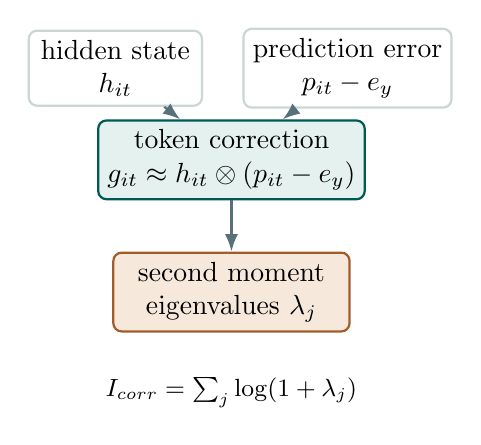
\begin{tikzpicture}[node distance=.35cm]
  \node[boxstyle,minimum width=2.2cm,minimum height=.9cm,align=center] (h) {hidden state\\$h_{it}$};
  \node[boxstyle,right=.5cm of h,minimum width=2.2cm,minimum height=.9cm,align=center] (e) {prediction error\\$p_{it}-e_y$};
  \node[tealbox,below=.65cm of $(h)!0.5!(e)$,minimum width=3.0cm,minimum height=.95cm,align=center] (g) {token correction\\$g_{it}\approx h_{it}\otimes(p_{it}-e_y)$};
  \draw[arr] (h)--(g);\draw[arr] (e)--(g);
  \node[amberbox,below=.65cm of g,minimum width=3.0cm,minimum height=.95cm,align=center] (S) {second moment\\eigenvalues $\lambda_j$};
  \draw[arr] (g)--(S);
  \node[below=.45cm of S,align=center,font=\small] {$I_{corr}=\sum_j\log(1+\lambda_j)$};
\end{tikzpicture}
\column{0.40\textwidth}
\vspace{0.35cm}
\stat{$\rho=0.764$}{within-model Spearman}
\vspace{0.55cm}
\small
22 conditions · 7 task families · 2 frozen 7B models
\vspace{0.35cm}
\begin{block}{Interpretation}
Large corrections in many independent directions tend to require a larger behavior-preserving update description.
\end{block}
\end{columns}
\vfill
\begin{center}\small\color{Muted}Promising campaign-level predictor; prospective validation still required.\end{center}
\note{\small\begin{itemize}
  \item Puisque le coût dépend du modèle, on regarde les corrections que chaque dataset demande à ce modèle.
  \item Le gradient token se factorise approximativement en état caché fois erreur de prédiction.
  \item On résume la diversité des directions de correction via le spectre d'un second moment.
  \item Le log-volume donne un Spearman within-model de 0.764 sur 22 conditions.
  \item Mais ce n'est pas encore une validation prospective indépendante.
\end{itemize}}
\end{frame}

\begin{frame}{Screening ten model-relative measures}
\framesubtitle{Ranking $R^*(0.90)$ within a model, and predicting a held-out task family}
\begin{center}\small
\setlength{\tabcolsep}{6pt}
\begin{tabular}{lrrrr}
\toprule
Measure & Within-model $\rho$ & Adjusted $p$ & Held-out RMSE & Pooled $\rho$\\
\midrule
Correction Fisher log-volume & \textbf{0.764} & \textbf{0.00034} & 0.187 & 0.584\\
Correction Fisher effective rank & 0.609 & 0.0112 & \textbf{0.181} & \textbf{0.814}\\
Surprise-weighted hidden log-volume & 0.614 & 0.0103 & 0.204 & 0.441\\
Base-model target code length & 0.200 & 0.524 & 0.261 & 0.269\\
Model-only fit & --- & --- & 0.264 & ---\\
\bottomrule
\end{tabular}
\end{center}
\vspace{0.25cm}
\begin{columns}[T,onlytextwidth]
\column{0.48\textwidth}
\small It follows the SQL/XBRL contrast: flat on SQL, rising on XBRL for both receivers.
\column{0.48\textwidth}
\small It is not learning gain under another name: correction log-volume and held-out gain correlate at $\rho=-0.275$.
\end{columns}
\note{\small\begin{itemize}
  \item Le log-volume de Fisher des corrections est notre meilleur prédicteur actuel.
  \item Il reproduit le contraste SQL/XBRL, ce qui est un bon signe de cohérence.
  \item Et il n'est pas un synonyme du gain appris: la corrélation avec le gain est négative.
\end{itemize}}
\end{frame}
% -----------------------------------------------------------------------------
% -----------------------------------------------------------------------------
\begin{frame}{Part I: what is established?}
\begin{columns}[T,onlytextwidth]
\column{0.49\textwidth}
\begin{block}{Operational definition}
\small A reloadable, serialized, behavior-based adapter rate relative to a fixed base model.
\end{block}
\begin{block}{Negative results}
\small Rank, raw dataset size, and weight RMSE are not sufficient notions of useful information.
\end{block}
\column{0.49\textwidth}
\begin{block}{Receiver dependence}
\small The same corpus changes cost when the frozen base model changes.
\end{block}
\begin{block}{Current hypothesis}
\small Model-relative correction geometry may predict the required rate.
\end{block}
\end{columns}
\vfill
\begin{center}\begin{minipage}{0.78\textwidth}\centering\Large\bfseries Information written by fine-tuning is not in the dataset alone.\end{minipage}\end{center}\vfill
\note{\small\begin{itemize}
  \item Résumé de la Partie I avant de changer d'objet.
  \item Contribution méthodologique: un taux exact, rechargeable et comportemental.
  \item Résultats négatifs: rang et RMSE ne suffisent pas.
  \item Résultat conceptuel le plus fort: changement de base model = changement du coût relatif.
  \item Hypothèse actuelle: prédire ce coût via la géométrie des corrections demandées au modèle.
\end{itemize}}
\end{frame}

% -----------------------------------------------------------------------------
\begin{frame}[plain]
  \begin{tikzpicture}[remember picture,overlay]\fill[Dark] (current page.south west) rectangle (current page.north east);\end{tikzpicture}
  \vspace{1.0cm}{\color{LightTeal}\bfseries PART II}\par\vspace{0.45cm}
  {\color{white}\fontsize{30}{33}\selectfont\bfseries Reasoning states}\par
  \vspace{0.55cm}{\color{white!72}\large At inference time, the information object is an intermediate state that should support future computation.}
  \note{\small\begin{itemize}
    \item Deuxième axe: à l'inférence, l'objet n'est plus une mise à jour de paramètres.
    \item On cherche un état intermédiaire qui permette de continuer le calcul.
    \item Il faut distinguer structure décodable, réutilisation causale et stabilité sous mises à jour répétées.
  \end{itemize}}
\end{frame}

% -----------------------------------------------------------------------------
\begin{frame}{Reasoning models still generate autoregressively}
\framesubtitle{Chain-of-thought changes the role of intermediate tokens, not the basic generation mechanism}
\begin{columns}[T,onlytextwidth]
\column{0.58\textwidth}
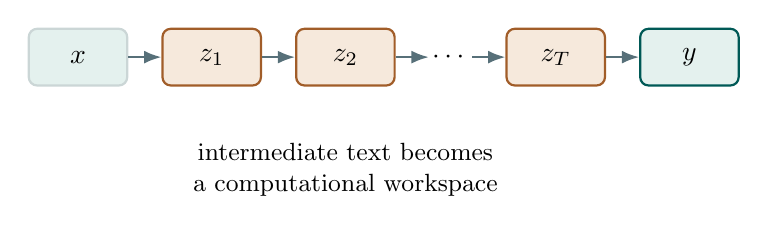
\begin{tikzpicture}[node distance=.22cm]
  \node[boxstyle,fill=Pale,minimum width=1.25cm,minimum height=.72cm] (x) {$x$};
  \node[amberbox,right=.42cm of x,minimum width=1.25cm,minimum height=.72cm] (z1) {$z_1$};
  \node[amberbox,right=.42cm of z1,minimum width=1.25cm,minimum height=.72cm] (z2) {$z_2$};
  \node[right=.42cm of z2,inner xsep=1pt] (dots) {$\cdots$};
  \node[amberbox,right=.42cm of dots,minimum width=1.25cm,minimum height=.72cm] (zt) {$z_T$};
  \node[tealbox,right=.42cm of zt,minimum width=1.25cm,minimum height=.72cm] (y) {$y$};
  \draw[arr] (x)--(z1);\draw[arr] (z1)--(z2);\draw[arr] (z2)--(dots);\draw[arr] (dots)--(zt);\draw[arr] (zt)--(y);
  \node[below=.6cm of z2,align=center,font=\small,text width=5cm] {intermediate text becomes a computational workspace};
\end{tikzpicture}
\vspace{0.35cm}
\[
p(z,y\mid x)=\Big[\prod_t p(z_t\mid x,z_{<t})\Big]p(y\mid x,z)
\]
\column{0.38\textwidth}
\small
\begin{itemize}\setlength\itemsep{6pt}
  \item CoT can improve multi-step reasoning \parencite{wei2022chain}
  \item RL-based post-training can induce long reasoning traces \parencite{shao2024deepseekmath,deepseekai2025r1}
  \item no architectural rule says semantic steps must align with sentence/token boundaries
\end{itemize}
\end{columns}
\note{\small\begin{itemize}
  \item Les reasoning models restent autoregressifs: un token après l'autre.
  \item Ce qui change, c'est la fonction des tokens intermédiaires: ils servent de workspace de calcul.
  \item CoT améliore plusieurs tâches, et le post-training moderne induit des traces longues sans démonstration explicite à l'inférence.
  \item Mais aucune contrainte architecturale n'aligne naturellement une étape sémantique avec une phrase ou un token précis.
\end{itemize}}
\end{frame}

% -----------------------------------------------------------------------------
\begin{frame}{Token trajectory $\neq$ reasoning-state trajectory}
\begin{columns}[T,onlytextwidth]
\column{0.54\textwidth}
\vspace{0.35cm}
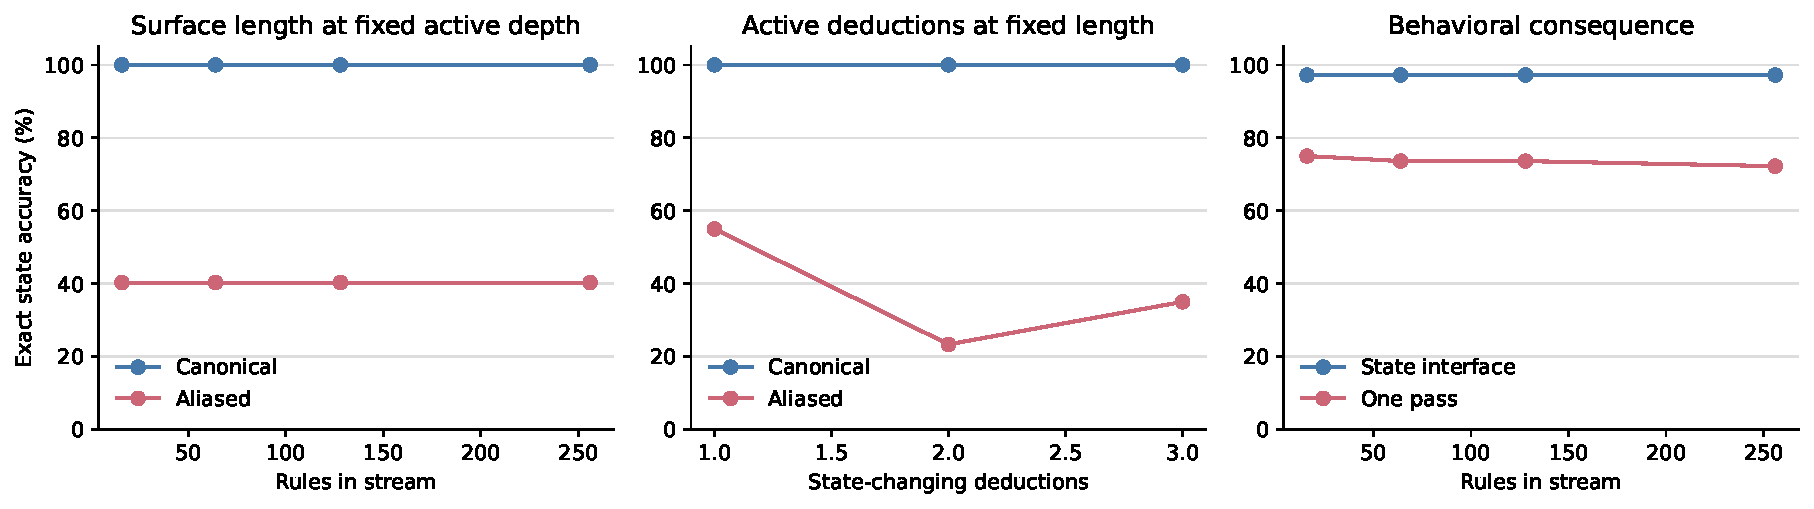
\includegraphics[width=\linewidth,trim=0bp 0bp 292bp 0bp,clip]{assets/real/depth_length.pdf}\par
\vspace{0.15cm}
{\footnotesize\color{Muted} surface token length vs.\ active deduction depth\par}
\column{0.42\textwidth}
\begin{block}{Candidate reasoning state}
\small A compact intermediate representation that is sufficient for a specified future computation.
\end{block}
\vspace{0.25cm}
\small
\textbf{Three increasingly strong claims}
\begin{enumerate}\setlength\itemsep{5pt}
  \item information is \key{decodable}
  \item state is \key{causally reusable}
  \item state remains sufficient under \key{repeated updates}
\end{enumerate}
\vfill\tinycite{dutta2024step,yang2025symbolic,sun2026trajectories}
\end{columns}
\note{\small\begin{itemize}
  \item On distingue le texte visible de la trajectoire d'activations internes.
  \item Une étape sémantique peut s'étaler sur de nombreux tokens, et un changement latent peut arriver sans ponctuation.
  \item Je définis donc un reasoning state par sa fonction: permettre une computation future spécifiée.
  \item Et je sépare trois niveaux: décodabilité, causalité, puis stabilité récursive.
\end{itemize}}
\end{frame}

\begin{frame}{The hypothesis we started from: a solution object}
\framesubtitle{A long derivation hiding a short series of stable updates}
\begin{columns}[T,onlytextwidth]
\column{0.52\textwidth}
\centering
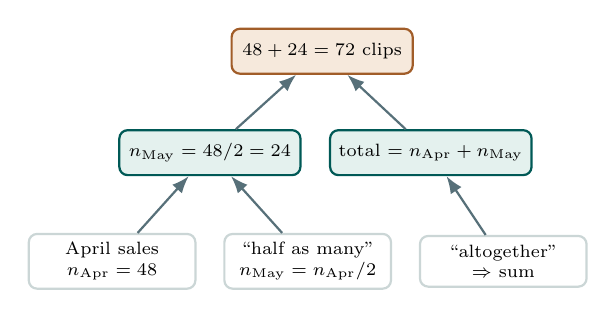
\begin{tikzpicture}[scale=.92,transform shape,font=\scriptsize]
  \node[boxstyle,minimum width=2.3cm,minimum height=.7cm,align=center] (f1) at (0,0) {April sales\\$n_{\mathrm{Apr}}=48$};
  \node[boxstyle,minimum width=2.3cm,minimum height=.7cm,align=center] (f2) at (2.7,0) {``half as many''\\$n_{\mathrm{May}}=n_{\mathrm{Apr}}/2$};
  \node[boxstyle,minimum width=2.3cm,minimum height=.7cm,align=center] (f3) at (5.4,0) {``altogether''\\$\Rightarrow$ sum};
  \node[tealbox,minimum width=2.5cm,minimum height=.62cm,align=center] (c1) at (1.35,1.5) {$n_{\mathrm{May}}=48/2=24$};
  \node[tealbox,minimum width=2.5cm,minimum height=.62cm,align=center] (c2) at (4.4,1.5) {total $=n_{\mathrm{Apr}}+n_{\mathrm{May}}$};
  \node[amberbox,minimum width=2.5cm,minimum height=.62cm,align=center] (sol) at (2.9,2.9) {$48+24=72$ clips};
  \draw[arr] (f1)--(c1);\draw[arr] (f2)--(c1);\draw[arr] (f3)--(c2);
  \draw[arr] (c1)--(sol);\draw[arr] (c2)--(sol);
\end{tikzpicture}
\column{0.44\textwidth}
\small
If such objects existed natively, several things should happen at the same places in a trace:
\begin{itemize}\setlength\itemsep{5pt}
  \item a meaningful text boundary coincides with a localized latent change
  \item equivalent computations permit causal transfer
  \item similar operations have similar representations
  \item those units help predict correctness
\end{itemize}
\end{columns}
\vfill
\begin{center}\begin{minipage}{0.9\textwidth}\centering\bfseries
So the first test is whether one partition of the trace can serve every one of those uses.
\end{minipage}\end{center}
\note{\small\begin{itemize}
  \item Hypothèse de départ: une longue chaîne de pensée suit un objet-solution compact.
  \item Les feuilles sont des lectures vérifiables de l'énoncé, les n\oe uds internes des opérations.
  \item Si cet objet existait nativement, plusieurs signaux devraient coïncider aux mêmes endroits.
\end{itemize}}
\end{frame}
% -----------------------------------------------------------------------------
\begin{frame}{Experiment: is there one utility-neutral partition of a trace?}
\framesubtitle{Same token gaps, same boundary budget, four objectives}
\begin{columns}[T,onlytextwidth]
\column{0.46\textwidth}
\begin{block}{Question}
Do the boundaries that are good for one use of a reasoning trace also serve the others?
\end{block}
\vspace{0.2cm}
\begin{block}{Why this design answers it}
\small Every trace gets the same number of boundaries, set by its count of verified symbolic updates, so no method can win by cutting more often. Random selection is normalized to 0 and each objective's own oracle to 1.
\end{block}
\column{0.46\textwidth}
\small
\textbf{Four objectives}
\begin{enumerate}\setlength\itemsep{4pt}
  \item representation moves toward the gold answer
  \item a verified symbolic update completes
  \item a held-out correctness probe changes
  \item local PCA geometry changes (compression signal)
\end{enumerate}
\vspace{0.25cm}
310{,}044 held-out SmolLM3-3B tokens; 61{,}691 Qwen3-14B tokens
\end{columns}
\note{\small\begin{itemize}
  \item Chaque intervalle entre deux tokens est un candidat frontière.
  \item Budget de frontières identique pour toutes les méthodes: personne ne gagne en coupant plus.
  \item Quatre utilités: réponse, mise à jour symbolique, correction, géométrie locale.
  \item Normalisation: aléatoire = 0, oracle de l'objectif = 1.
\end{itemize}}
\end{frame}
% -----------------------------------------------------------------------------
% -----------------------------------------------------------------------------
\begin{frame}{Different utilities select different boundaries}
\framesubtitle{Same token gaps, same boundary budget, four objectives}
\begin{columns}[T,onlytextwidth]
\column{0.58\textwidth}
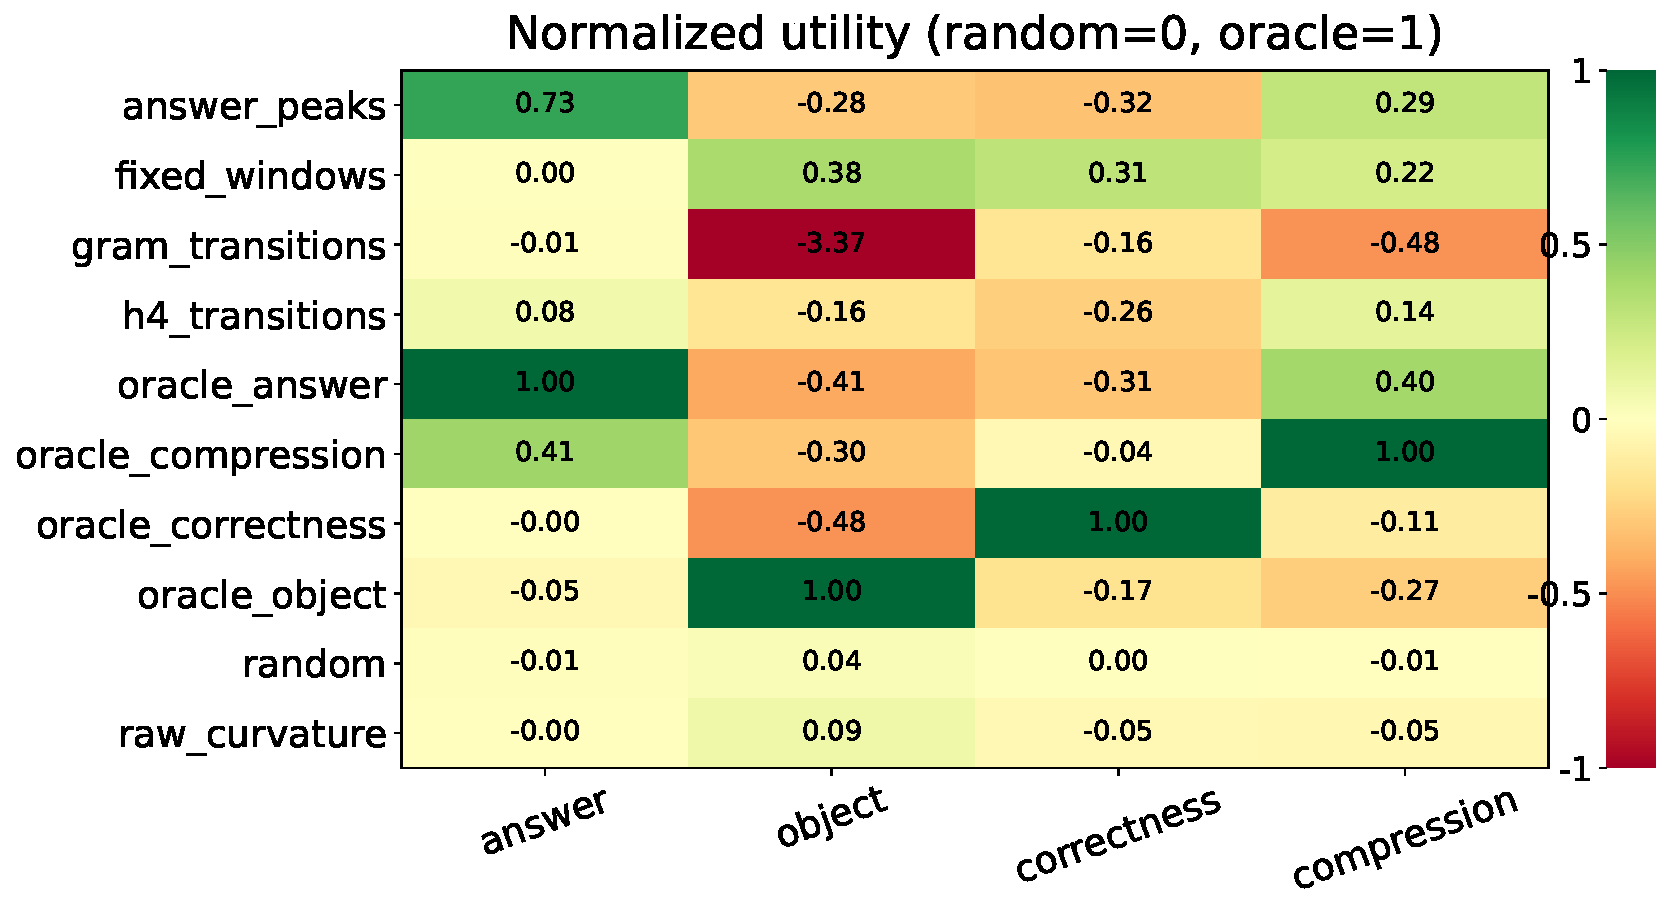
\includegraphics[width=0.92\linewidth,trim=0bp 0bp 0bp 30bp,clip]{assets/real/objective_matrix.pdf}
\par\vspace{0.3cm}
{\small Supervised detectors recover each target well, but the target-specific oracle partitions barely overlap.\par}
\column{0.38\textwidth}
\stat{0.098--0.210}{oracle-boundary F1 within $\pm4$ tokens}
\vspace{0.55cm}
\stat{0.020}{best worst-objective utility}
\vspace{0.45cm}
\small Primary SmolLM experiment.
\end{columns}
\vspace{0.1cm}
\begin{center}\bfseries Structure is decodable; a utility-independent partition is not.\end{center}
\tinycite{qian2025peaks,yu2025stateaware,sun2026trajectories}
\note{\small\begin{itemize}
  \item Quatre objectifs sur exactement les mêmes gaps entre tokens, avec le même budget de frontières.
  \item Les détecteurs supervisés retrouvent très bien leur propre cible: il y a donc du signal.
  \item Mais les oracles spécifiques se recouvrent très peu: F1 environ 0.10 à 0.21.
  \item La meilleure règle testée pour servir tous les objectifs atteint seulement 0.020 en worst-objective utility.
  \item Conclusion: pas d'absence de structure; absence d'une structure unique indépendante de l'usage.
\end{itemize}}
\end{frame}

\begin{frame}{Decodable, but not one structure}
\framesubtitle{Regret against each objective's own oracle}
\begin{columns}[T,onlytextwidth]
\column{0.52\textwidth}
\centering
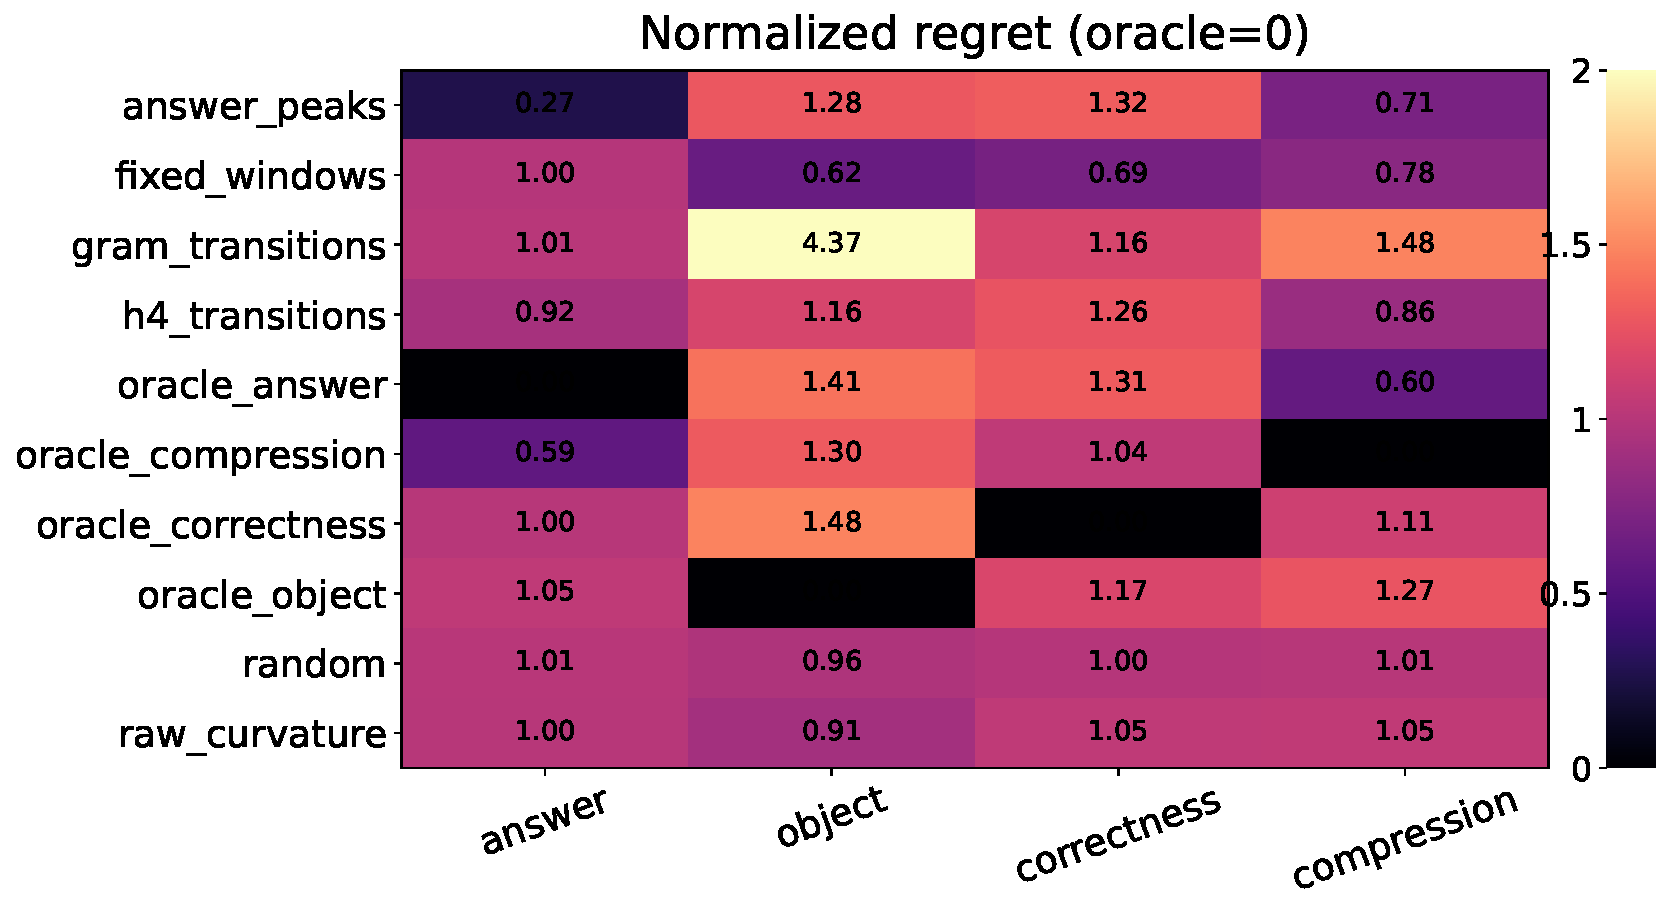
\includegraphics[width=\linewidth,trim=0bp 0bp 0bp 30bp,clip]{assets/real/regret_matrix.pdf}
\column{0.44\textwidth}
\small
\textbf{Supervised detectors recover their own target}\par
\vspace{4pt}
held-out ROC--AUC, SmolLM: {\color{Teal}\bfseries 0.999 / 0.984 / 0.849 / 0.868}\par
\vspace{2pt}
Qwen: {\color{Teal}\bfseries 0.998 / 0.992 / 0.859 / 0.825}\par
\vspace{0.3cm}
\textbf{But they select different partitions}\par
\vspace{4pt}
cross-objective F1 within 4 tokens: 0.098--0.210 (SmolLM), 0.130--0.294 (Qwen)\par
\vspace{2pt}
best worst-objective utility: 0.020 (SmolLM), 0.080 (Qwen)
\end{columns}
\vspace{0.1cm}
\begin{center}\begin{minipage}{0.92\textwidth}\centering\bfseries
Not an absence of latent structure --- an absence of one utility-independent structure.
\end{minipage}\end{center}
\note{\small\begin{itemize}
  \item Les détecteurs supervisés retrouvent très bien leur propre cible: le signal existe.
  \item Mais le transfert entre objectifs est faible, et aucune règle ne sert les quatre.
  \item Le projet passe donc de « trouver la partition canonique » à « quel état suffit pour quel usage ».
\end{itemize}}
\end{frame}
% -----------------------------------------------------------------------------
\begin{frame}{Objection: maybe the four objectives missed the semantic steps}
\framesubtitle{Judged spans as a human-facing control}
\begin{columns}[T,onlytextwidth]
\column{0.46\textwidth}
\begin{block}{Question}
Would boundaries that a human reader would call reasoning steps behave differently?
\end{block}
\vspace{0.2cm}
\begin{block}{Why this design answers it}
\small The labels come from outside our four operational objectives, so agreement or disagreement with them is independent evidence.
\end{block}
\column{0.46\textwidth}
\small
\textbf{Setup}
\begin{itemize}\setlength\itemsep{4pt}
  \item Qwen-110B-A25B as judge over 415 overlapping windows of concise correct SmolLM traces
  \item nine edit types: orient, bind variable, add relation, derive value, verify, correct error, plan, extract answer, mixed
  \item after alignment and edge filtering: 1{,}761 spans over 58 traces, median 29 tokens
  \item latent detector trained question-disjoint
\end{itemize}
\end{columns}
\note{\small\begin{itemize}
  \item Contrôle contre une objection naturelle sur le choix des objectifs.
  \item Un grand modèle juge annote neuf types d'édition sur des fenêtres chevauchantes.
  \item Split question-disjoint: on ne peut pas mémoriser les mêmes problèmes.
\end{itemize}}
\end{frame}
% -----------------------------------------------------------------------------
% -----------------------------------------------------------------------------
\begin{frame}{Readable semantic spans are decodable too --- but still objective-relative}
\begin{columns}[T,onlytextwidth]
\column{0.55\textwidth}
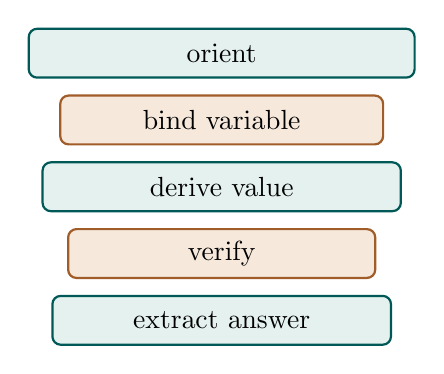
\begin{tikzpicture}[node distance=.27cm]
  \node[tealbox,minimum width=4.9cm,minimum height=.62cm] (a) {orient};
  \node[amberbox,below=.2cm of a,minimum width=4.1cm,minimum height=.62cm] (b) {bind variable};
  \node[tealbox,below=.2cm of b,minimum width=4.55cm,minimum height=.62cm] (c) {derive value};
  \node[amberbox,below=.2cm of c,minimum width=3.9cm,minimum height=.62cm] (d) {verify};
  \node[tealbox,below=.2cm of d,minimum width=4.3cm,minimum height=.62cm] (e) {extract answer};
\end{tikzpicture}
\column{0.41\textwidth}
\stat{0.982}{latent boundary AUC}
\vspace{0.35cm}
\stat{0.969}{away from sentence endings}
\vspace{0.35cm}
\stat{0.892}{lexical TF--IDF baseline}
\end{columns}
\vfill
\small\centering 1,761 judged spans over 58 traces; transfer to the four operational objectives remains weak.
\note{\small\begin{itemize}
  \item Contrôle contre une objection naturelle: nos quatre objectifs opérationnels ont peut-être raté les « vraies » étapes sémantiques.
  \item Un grand modèle étiquette neuf types d'édition; on obtient 1 761 spans.
  \item Les frontières sont très décodables dans les activations, même loin des fins de phrase.
  \item Mais un baseline lexical est déjà fort, et surtout ces frontières transfèrent mal vers les quatre utilités précédentes.
\end{itemize}}
\end{frame}

\begin{frame}{Experiment: is snapshot information the same thing as memory?}
\framesubtitle{An exact finite control, with no generation or judging noise}
\begin{columns}[T,onlytextwidth]
\column{0.46\textwidth}
\begin{block}{Question}
Can two representations carry the same information now and still differ as memories later?
\end{block}
\vspace{0.2cm}
\begin{block}{Why this design answers it}
\small The hidden-state model, the memory update and the planner are all explicit, so any performance difference is attributable to the representation and its update rule.
\end{block}
\column{0.46\textwidth}
\small
\textbf{Setup}
\begin{itemize}\setlength\itemsep{4pt}
  \item controller observes a short history from a finite hidden state, then decides over a future horizon
  \item memories: full public history, 12-bit text suffix, 12-bit explicit field state, no memory
  \item 90 task cells
  \item matched at the start: same support, $I(S;M)=2.512$ bits, path leakage 1.781 bits
\end{itemize}
\end{columns}
\note{\small\begin{itemize}
  \item Contrôle fini exact: pas de bruit de génération ni de juge.
  \item Les représentations partent avec exactement la même information sur l'état.
  \item Toute différence ultérieure vient donc de la règle de mise à jour.
\end{itemize}}
\end{frame}
% -----------------------------------------------------------------------------
% -----------------------------------------------------------------------------
\begin{frame}{Snapshot information is not memory}
\framesubtitle{Exact finite control: same initial information, different update rule}
\begin{columns}[T,onlytextwidth]
\column{0.98\textwidth}\centering
\resizebox{\linewidth}{!}{%
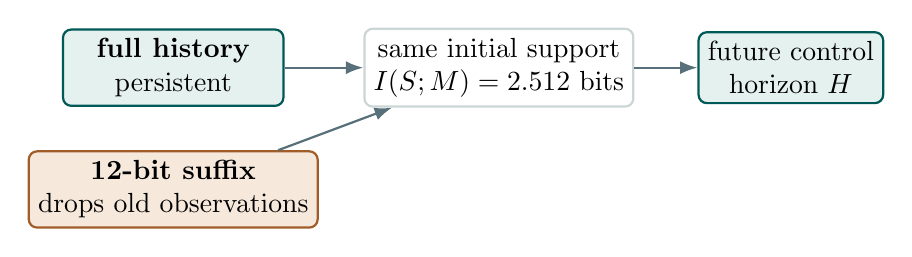
\begin{tikzpicture}[node distance=.3cm]
  \node[tealbox,minimum width=2.8cm,minimum height=.9cm,align=center] (full) {\bfseries full history\\persistent};
  \node[amberbox,below=.55cm of full,minimum width=2.8cm,minimum height=.9cm,align=center] (suf) {\bfseries 12-bit suffix\\drops old observations};
  \node[boxstyle,right=1.0cm of full,minimum width=3.2cm,minimum height=.9cm,align=center] (same) {same initial support\\$I(S;M)=2.512$ bits};
  \draw[arr] (full)--(same);\draw[arr] (suf)--(same);
  \node[tealbox,right=.8cm of same,minimum width=2.2cm,minimum height=.9cm,align=center] (future) {future control\\horizon $H$};
  \draw[arr] (same)--(future);
\end{tikzpicture}}
\end{columns}
\vfill
\begin{center}\bfseries A reusable state must be sufficient \emph{and remain sufficient after updates}.\end{center}
\note{\small\begin{itemize}
  \item Contrôle fini exact: pas de bruit de génération LLM.
  \item Full history et suffixe 12 bits commencent avec le même support et la même information instantanée sur l'état.
  \item La différence apparaît ensuite parce que le suffixe oublie les observations anciennes.
  \item À horizon 32, regret 2.20 contre 30.91.
  \item Donc une mesure snapshot ne suffit pas à définir une mémoire utile; l'update rule fait partie du récepteur.
\end{itemize}}
\end{frame}

\begin{frame}{Equal snapshot information, unequal memory}
\framesubtitle{Exact closed-loop regret over the continuation horizon}
\begin{columns}[T,onlytextwidth]
\column{0.60\textwidth}
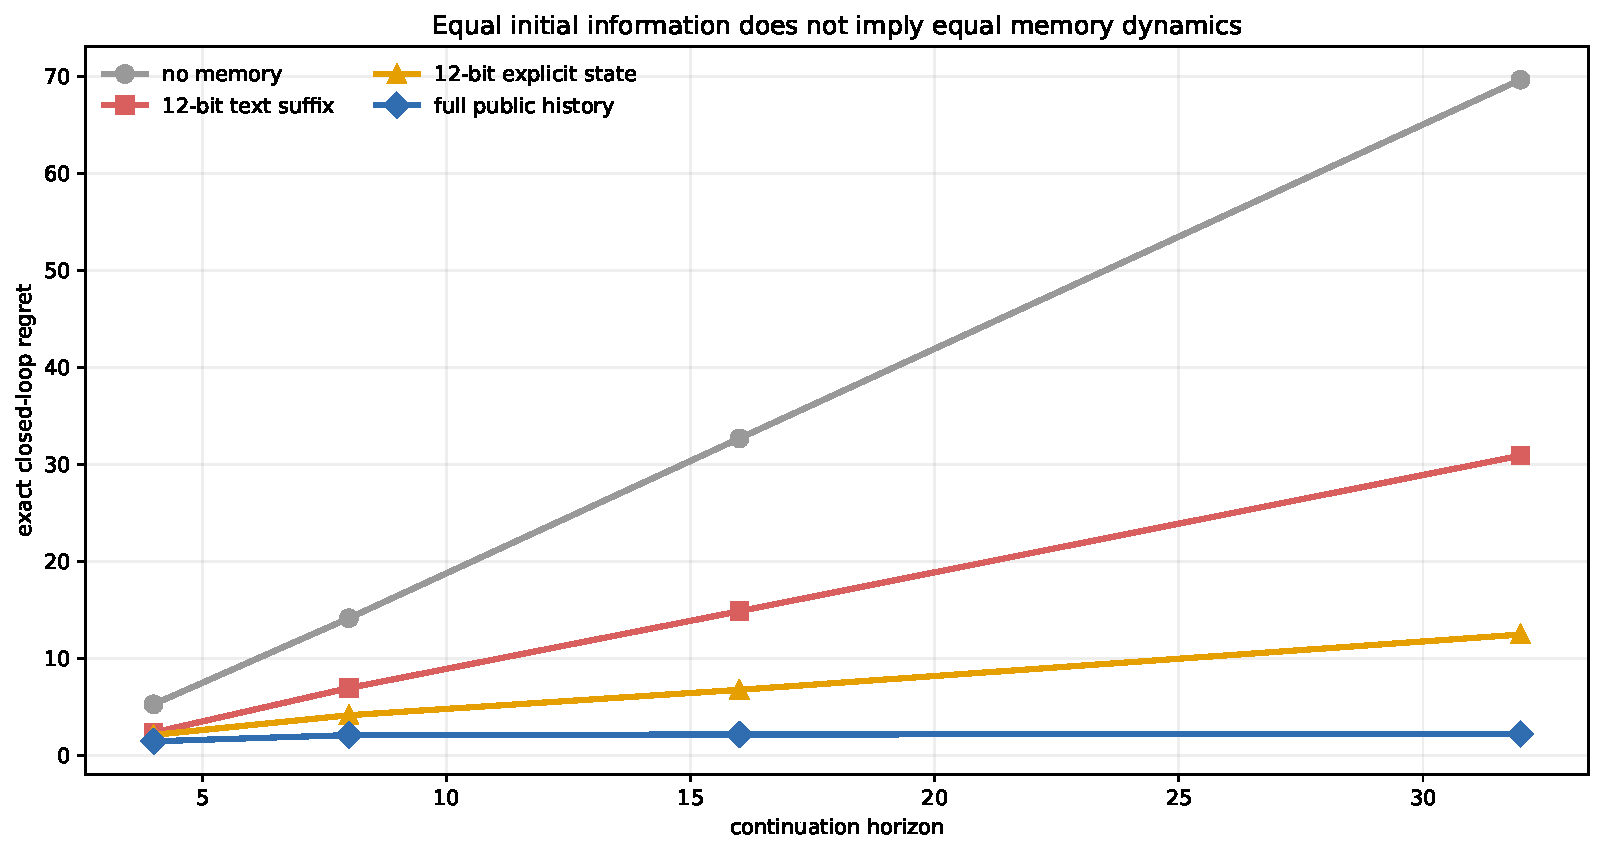
\includegraphics[width=\linewidth,trim=0bp 0bp 0bp 24bp,clip]{assets/real/closed_loop_regret.pdf}
\column{0.36\textwidth}
\vspace{0.3cm}
\stat{$7.19\times$}{pooled regret, suffix vs.\ full history}
\vspace{0.3cm}
\small
\begin{itemize}\setlength\itemsep{5pt}
  \item at $H=32$: {\color{Teal}\bfseries 2.20} full history, {\color{Teal}\bfseries 30.91} suffix
  \item regret removed vs.\ no memory: 93.7\% full history, 79.3\% field state, 54.8\% suffix
\end{itemize}
\end{columns}
\vspace{0.1cm}
\begin{center}\begin{minipage}{0.92\textwidth}\centering\bfseries
Matched initial capacity rules out capacity: the gap appears only as the memories are updated.
\end{minipage}\end{center}
\note{\small\begin{itemize}
  \item Même support initial, même information mutuelle, et pourtant jamais le même regret.
  \item À l'horizon 32: 2.20 pour l'historique complet contre 30.91 pour le suffixe.
  \item L'état explicite 12 bits fait beaucoup mieux que le suffixe, sans égaler l'historique.
  \item Le suffixe échoue parce qu'il oublie les observations anciennes au fil des mises à jour.
\end{itemize}}
\end{frame}
% -----------------------------------------------------------------------------
\begin{frame}{Experiment: can a frozen model route its own state?}
\framesubtitle{Synthetic addition task where the needed intermediate state is known exactly}
\begin{columns}[T,onlytextwidth]
\column{0.46\textwidth}
\begin{block}{Question}
Is failure at multi-step composition a failure to \emph{infer} the state, or a failure to \emph{use} it?
\end{block}
\vspace{0.2cm}
\begin{block}{Why this design answers it}
\small A short program leads to one of eight three-bit states and a separate table maps that state to the answer, so reading, updating, inferring and using the state can each be scored separately.
\end{block}
\column{0.46\textwidth}
\small
\textbf{Four abilities tested separately}
\begin{enumerate}\setlength\itemsep{4pt}
  \item read a supplied state
  \item apply a local update
  \item infer the endpoint of a history
  \item use that inferred endpoint in the final lookup
\end{enumerate}
\vspace{0.25cm}
frozen Qwen2.5-32B; eight-state chance level is 12.5\%
\end{columns}
\note{\small\begin{itemize}
  \item Tâche synthétique où l'état intermédiaire nécessaire est connu exactement.
  \item On sépare quatre capacités: lire, mettre à jour, inférer, puis utiliser l'état inféré.
  \item Le niveau de chance est 12.5\% avec huit états.
\end{itemize}}
\end{frame}
% -----------------------------------------------------------------------------
% -----------------------------------------------------------------------------
\begin{frame}{Explicit handoff restores composition}
\framesubtitle{Controlled eight-state program with frozen Qwen2.5-32B}
\begin{center}
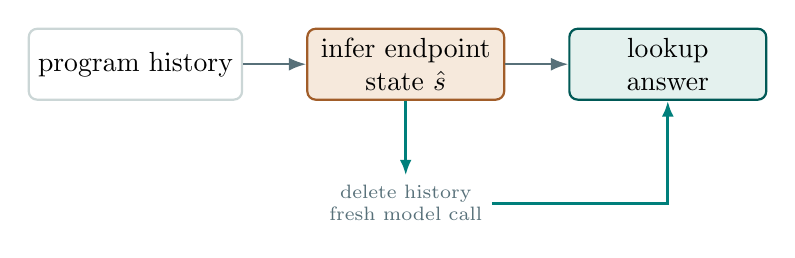
\begin{tikzpicture}[node distance=.33cm]
  \node[boxstyle,minimum width=2.6cm,minimum height=.9cm,align=center] (hist) {program history};
  \node[amberbox,right=.8cm of hist,minimum width=2.5cm,minimum height=.9cm,align=center] (infer) {infer endpoint\\state $\hat s$};
  \node[tealbox,right=.8cm of infer,minimum width=2.5cm,minimum height=.9cm,align=center] (look) {lookup\\answer};
  \draw[arr] (hist)--(infer);\draw[arr] (infer)--(look);
  \node[below=.95cm of infer,align=center,font=\scriptsize,text=Muted] (fresh) {delete history\\fresh model call};
  \draw[-{Latex[length=2mm]},draw=Teal,line width=1.1pt] (infer.south)--(fresh.north);
  \draw[-{Latex[length=2mm]},draw=Teal,line width=1.1pt] (fresh.east) -| (look.south);
\end{tikzpicture}
\end{center}
\vspace{0.45cm}
\begin{center}
\small
\begin{tabular}{lr}
\toprule
assay & accuracy\\\midrule
one-pass infer+lookup & 13.44\%\\
endpoint inference & 76.98\%\\
explicit handoff & 76.98\%\\
correct endpoint given & 100\%\\
\bottomrule
\end{tabular}
\end{center}
\vfill
\begin{center}\bfseries The missing ingredient can be routing/composition, not missing state information.\end{center}
\note{\small\begin{itemize}
  \item Assay contrôlé à huit états: historique de programme puis table state-to-answer.
  \item Le modèle sait inférer l'endpoint à environ 77\%, mais le one-pass endpoint+lookup tombe à 13.44\%.
  \item Intervention: faire prédire l'état, supprimer l'historique, donner uniquement cet état à un nouvel appel.
  \item La précision revient exactement à 76.98\%; endpoint correct fourni donne 100\%.
  \item Cela isole un problème de routage/composition plutôt qu'une simple absence d'information.
\end{itemize}}
\end{frame}

\begin{frame}{Experiment: what makes a supplied interface work?}
\framesubtitle{Finite proof task, four code designs at equal data and compute}
\begin{columns}[T,onlytextwidth]
\column{0.46\textwidth}
\begin{block}{Question}
Is enough capacity sufficient for a reusable state code, or does the naming matter too?
\end{block}
\vspace{0.2cm}
\begin{block}{Why this design answers it}
\small At each step the previous rules are discarded and only the state code is passed on, so the experiment succeeds only if the code itself carries the state.
\end{block}
\column{0.46\textwidth}
\small
\textbf{Four codes, one four-bit fact ledger (16 states)}
\begin{itemize}\setlength\itemsep{4pt}
  \item \key{3-bit lossy}: must merge some states
  \item \key{4-bit canonical}: one stable name per state
  \item \key{5-bit padded}: unused capacity, still one name
  \item \key{5-bit path-aliased}: same state, two names depending on the path
\end{itemize}
\vspace{0.2cm}
the last pair isolates capacity from naming
\end{columns}
\note{\small\begin{itemize}
  \item Tâche de preuve finie: un registre de quatre faits, donc seize états.
  \item À chaque étape, seules les règles courantes et le code d'état sont transmis.
  \item Les quatre codes séparent capacité insuffisante, capacité en excès et nommage instable.
\end{itemize}}
\end{frame}
% -----------------------------------------------------------------------------
% -----------------------------------------------------------------------------
\begin{frame}{Capacity and stable names are separate requirements}
\begin{columns}[T,onlytextwidth]
\column{0.55\textwidth}
\vspace{0.2cm}
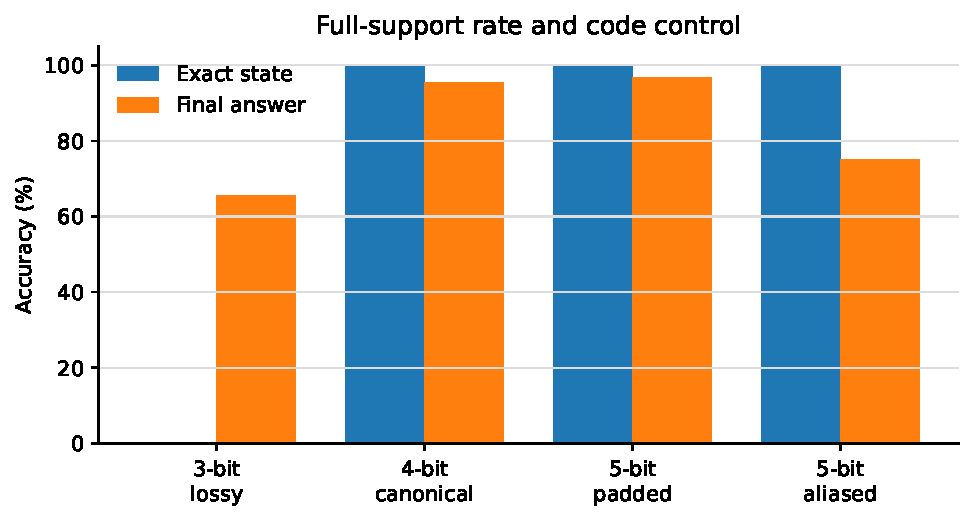
\includegraphics[width=\linewidth,trim=0bp 0bp 0bp 20bp,clip]{assets/real/rate_sufficiency.pdf}\par
\vspace{0.1cm}
{\footnotesize canonical interface 97.22\% vs.\ 72.22\% one-pass reasoning; paired gain 25 points, CI $[12.50,38.89]$\par}
\column{0.41\textwidth}
\small
\begin{itemize}\setlength\itemsep{7pt}
  \item 3 bits: unavoidable collisions
  \item 4-bit canonical: exact through $H=256$
  \item 5-bit padded: exact through $H=256$
  \item 5-bit path-aliased: $30$--$40\%$ by depth 3
\end{itemize}
\end{columns}
\vfill
\begin{center}\bfseries Same capacity $\neq$ same causal interface. Shared semantics must be stable.\end{center}
\note{\small\begin{itemize}
  \item On sépare ici capacité brute et sémantique de l'interface.
  \item 16 états demandent au moins 4 bits pour une identification exacte.
  \item 4-bit canonical et 5-bit padded gardent un nom stable par état et restent exacts très loin.
  \item 5-bit path-aliased a plus de capacité mais plusieurs noms pour le même état selon l'historique; les performances chutent très vite.
  \item Donc le nombre de bits seul ne suffit pas: le code doit avoir une sémantique partagée et stable.
\end{itemize}}
\end{frame}

% -----------------------------------------------------------------------------
\begin{frame}{Local competence can collapse under recursive use}
\begin{columns}[T,onlytextwidth]
\column{0.60\textwidth}
\vspace{0.25cm}
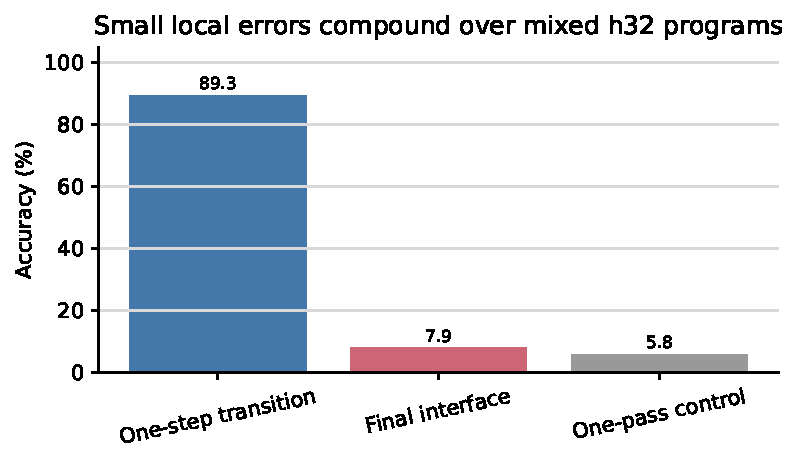
\includegraphics[width=0.96\linewidth]{assets/real/06_local_global_reliability.pdf}
\column{0.36\textwidth}
\stat{$\approx89\%$}{correct local transitions}
\vspace{0.45cm}
\stat{7.92\%}{correct final answer at $H=32$}
\end{columns}
\vfill
\begin{center}\small Chance: 6.25\% · one-pass reasoning: 5.83\%\end{center}
\vspace{0.25cm}
\begin{center}\bfseries Closed-loop reliability is a property of the state \emph{and} its update dynamics.\end{center}
\note{\small\begin{itemize}
  \item Sur une tâche register plus variée, la transition locale est correcte environ 89\% du temps.
  \item Mais en réinjectant les états prédits sur 32 étapes, la réponse finale tombe à 7.92\%, quasiment chance.
  \item Le test local repart toujours de l'état réellement fourni: il ne double-compte pas les erreurs antérieures.
  \item Moralité: une interface peut sembler bonne localement et être inutilisable en boucle fermée.
\end{itemize}}
\end{frame}

\begin{frame}{The present limit of the interface approach}
\begin{columns}[T,onlytextwidth]
\column{0.48\textwidth}
\begin{block}{What the gap separates}
\small Local transition competence, scored from the state actually supplied at each call, from accumulated reliability under self-conditioned use.
\end{block}
\column{0.48\textwidth}
\begin{block}{What was ruled out as a fix}
\small The pattern was not model-dependent, and adding a fifth code bit did not repair it.
\end{block}
\end{columns}
\vfill
\begin{center}\begin{minipage}{0.92\textwidth}\centering\bfseries
A transition function that is 89\% correct in one step is not reliable enough for dozens of recursive uses --- a horizon reasoning models reach easily.
\end{minipage}\end{center}
\vspace{0.2cm}
\begin{center}\small Long-horizon reliability has to be measured under self-conditioned use, not inferred from gold-input one-step accuracy.\end{center}
\note{\small\begin{itemize}
  \item C'est la limite actuelle de l'approche par interface explicite.
  \item Ni le choix du modèle ni un bit de code supplémentaire ne réparent le problème.
  \item Les petites erreurs sémantiques se composent jusqu'à rendre l'état inutilisable.
\end{itemize}}
\end{frame}
% -----------------------------------------------------------------------------
\begin{frame}{Experiment: do reasoning and answer cost the same to write?}
\framesubtitle{The first bridge between the two parts}
\begin{columns}[T,onlytextwidth]
\column{0.46\textwidth}
\begin{block}{Question}
Within one adapter, does the reasoning chain require more update information than the final answer?
\end{block}
\vspace{0.2cm}
\begin{block}{Why this design answers it}
\small Same corpus, same codec ladder and same rate axis as Part I; only the supervised span and the frozen receiver change.
\end{block}
\column{0.46\textwidth}
\small
\textbf{Setup}
\begin{itemize}\setlength\itemsep{4pt}
  \item rank-16 all-linear LoRA on MetaMathQA
  \item two frozen NF4 backbones: Mistral-7B, Qwen2.5-7B
  \item three supervisions: full response, reasoning span only, answer span only
  \item scored separately on reasoning and answer spans
\end{itemize}
\vspace{0.2cm}
$R^{\star}_{M,U}(\tau)=\min_A R(A)$ s.t.\ $W_{M,U}(A)\ge\tau W_{M,U}(A_{\mathrm{raw}})$
\end{columns}
\note{\small\begin{itemize}
  \item Même protocole de compression que la partie I, appliqué à des spans différents.
  \item Trois supervisions: réponse complète, raisonnement seul, réponse finale seule.
  \item Le taux est mesuré séparément pour chaque utilité de span.
\end{itemize}}
\end{frame}
% -----------------------------------------------------------------------------
% -----------------------------------------------------------------------------
\begin{frame}{The two axes meet: even reasoning-vs-answer rate is receiver-dependent}
\framesubtitle{Same MetaMathQA adapters; same codec; two utilities}
\begin{columns}[T,onlytextwidth]
\column{0.62\textwidth}
\vspace{0.05cm}
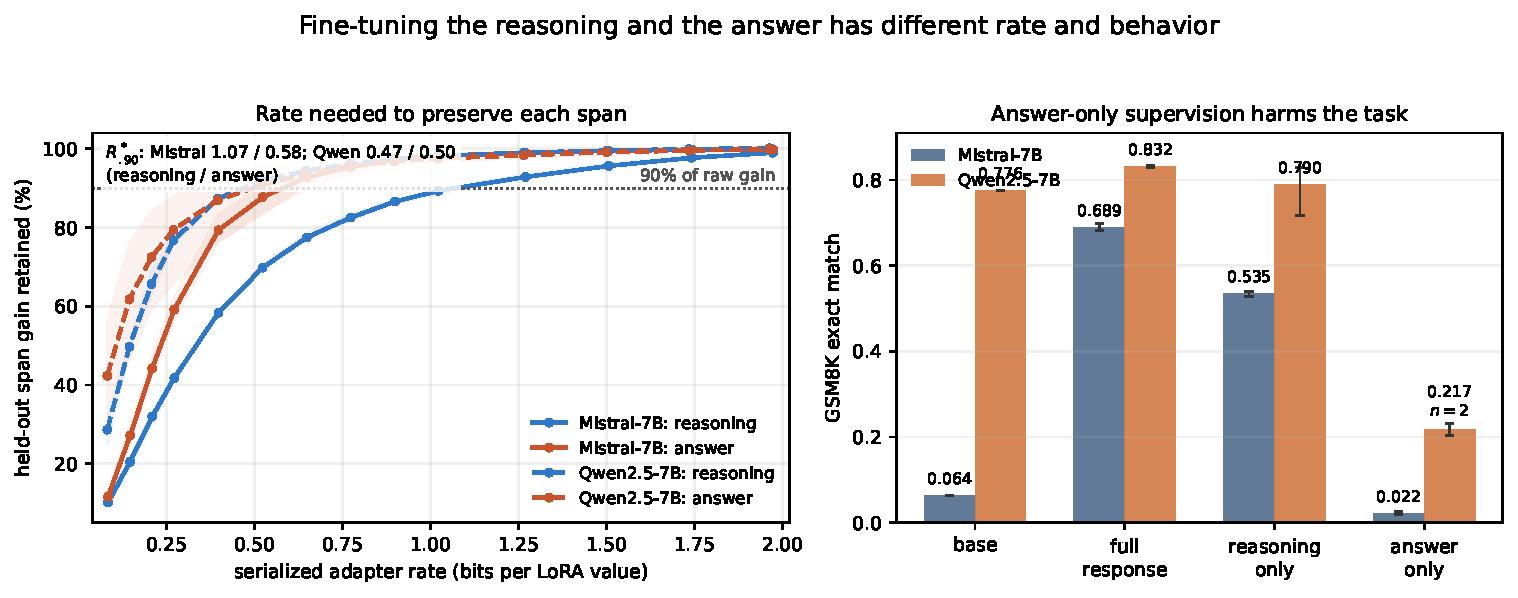
\includegraphics[width=0.80\linewidth,trim=0bp 0bp 348bp 20bp,clip]{assets/real/cot_finetuning_limits.pdf}
\column{0.34\textwidth}
\small
\textbf{Ordering reverses}
\vspace{0.3cm}
\begin{itemize}\setlength\itemsep{7pt}
  \item Mistral: reasoning costs much more
  \item Qwen: reasoning costs slightly less
  \item answer rates almost match
\end{itemize}
\end{columns}
\vspace{0.15cm}
\begin{center}\bfseries Utility and receiver jointly define the update information we measure.\end{center}
\note{\small\begin{itemize}
  \item Connexion directe entre les deux axes: même protocole de compression d'adapter, mais scoring séparé des tokens de reasoning et de réponse.
  \item Mistral: reasoning 1.070 bits/value, answer 0.578.
  \item Qwen: reasoning 0.471, answer 0.575: l'ordre s'inverse.
  \item Attention: c'est un taux de stockage d'update, pas une mesure de longueur informationnelle intrinsèque de la CoT.
\end{itemize}}
\end{frame}

% -----------------------------------------------------------------------------
\begin{frame}{Unified interpretation}
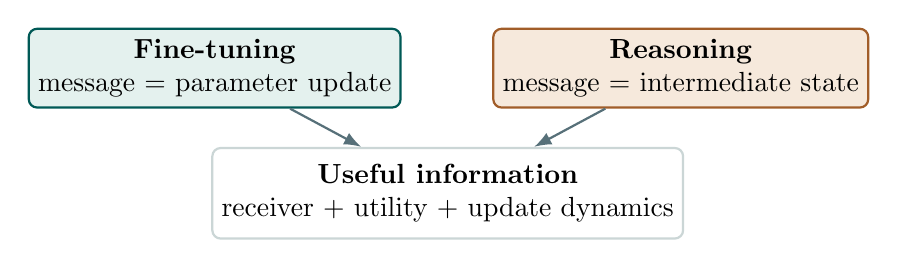
\begin{tikzpicture}[node distance=.55cm]
  \node[tealbox,minimum width=4.1cm,minimum height=1.0cm,align=center] (ft) {\bfseries Fine-tuning\\message = parameter update};
  \node[amberbox,right=1.15cm of ft,minimum width=4.1cm,minimum height=1.0cm,align=center] (rs) {\bfseries Reasoning\\message = intermediate state};
  \node[boxstyle,below=1.0cm of $(ft)!0.5!(rs)$,minimum width=4.5cm,minimum height=1.15cm,align=center] (common) {\bfseries Useful information\\receiver + utility + update dynamics};
  \draw[arr] (ft)--(common);\draw[arr] (rs)--(common);
\end{tikzpicture}
\vspace{0.55cm}
\begin{columns}[T,onlytextwidth]
\column{0.48\textwidth}
\textbf{Established}
\begin{itemize}\small
  \item receiver-dependent adapter rate
  \item objective-dependent reasoning partitions
  \item decodable $\not\Rightarrow$ reusable
  \item local $\not\Rightarrow$ recursively reliable
\end{itemize}
\column{0.48\textwidth}
\textbf{Next falsifiable tests}
\begin{itemize}\small
  \item predict $R^*$ prospectively from correction spectra
  \item compress a reasoning adapter and locate which behavior fails first
\end{itemize}
\end{columns}
\note{\small\begin{itemize}
  \item Lecture commune: l'information utile n'est pas dans l'objet seul.
  \item Fine-tuning: elle est relative au base model qui décode l'update et à la métrique qu'on veut préserver.
  \item Reasoning: elle est relative à l'opération future et, sous récursion, à la règle de mise à jour.
  \item On n'a pas encore une loi prédictive unique reliant les deux axes; le pont est conceptuel et expérimental.
\end{itemize}}
\end{frame}

% -----------------------------------------------------------------------------
\begin{frame}[plain]
  \begin{tikzpicture}[remember picture,overlay]\fill[Dark] (current page.south west) rectangle (current page.north east);\end{tikzpicture}
  \vspace{1.25cm}
  {\color{LightTeal}\bfseries CONCLUSION}\par\vspace{0.6cm}
  {\color{white}\fontsize{31}{34}\selectfont\bfseries Useful information depends on its use}\par
  \vspace{0.9cm}
  \begin{columns}[T,onlytextwidth]
  \column{0.48\textwidth}{\color{white}\bfseries Receiver}\par{\color{white!72}\small Which model must use the information?}
  \column{0.48\textwidth}{\color{white}\bfseries Utility + update rule}\par{\color{white!72}\small Which behavior must survive, and for how long?}
  \end{columns}
  \vspace{1.15cm}
  {\color{white}\large Information is not in the object alone; it is in the object-for-a-use.}
  \note{\small\begin{itemize}
    \item Contribution centrale: remplacer des proxies vagues par des tests comportementaux concrets.
    \item Fine-tuning: message supplémentaire nécessaire à un base model donné.
    \item Reasoning: état qui permet réellement de continuer le calcul.
    \item Dans les deux cas, receiver + utility définissent ce qui compte; sous répétition, l'update rule s'ajoute.
    \item Phrase finale puis merci.
  \end{itemize}}
\end{frame}


% -----------------------------------------------------------------------------
\begin{frame}[allowframebreaks]{References used in the presentation}
\printbibliography[heading=none]
\end{frame}

% ============================== BACKUP =======================================
\appendix

% -----------------------------------------------------------------------------
\begin{frame}{Backup: codec contract}
\begin{columns}[T,onlytextwidth]
\column{0.48\textwidth}
\begin{block}{Included in the file}
\small
\begin{itemize}
  \item quantized LoRA factors
  \item scales and metadata
  \item bit-packed payload
  \item zlib compression
\end{itemize}
\end{block}
\column{0.48\textwidth}
\begin{block}{Conditioned on}
\small
\begin{itemize}
  \item shared frozen base model
  \item fixed adapter layout/checkpoint
  \item named held-out utility
  \item decoder implementation
\end{itemize}
\end{block}
\end{columns}
\vfill
\begin{center}\bfseries $R^*$ is attainable within the tested codec family, not a global description-length optimum.\end{center}
\note{\small\begin{itemize}
  \item Rappeler ce qui compte ou non dans le budget.
  \item Le base model est explicitement hors budget car partagé.
  \item Comparer des rangs différents demande aussi la taille totale du fichier, pas seulement bits/value.
\end{itemize}}
\end{frame}

\begin{frame}{Backup: metric definitions}
\small
\begin{tabular}{p{.25\textwidth}p{.65\textwidth}}
\toprule
Metric & Question answered\\\midrule
NLL / bits per token & How well does the model predict the held-out continuation?\\
Exact match & Is the final discrete answer correct?\\
Retained gain & How much of the raw adapter's improvement survives compression?\\
Boundary AUC/F1 & Is a target boundary decodable / selected at the right locations?\\
Exact state & Is the complete finite-state ledger correct?\\
\bottomrule
\end{tabular}
\vfill
\begin{center}\bfseries 90\% retained NLL gain does not mean 90\% final-answer accuracy.\end{center}
\note{\small\begin{itemize}
  \item Les métriques répondent à des questions différentes.
  \item Retained gain doit toujours nommer l'utility sous-jacente.
  \item AUC = ranking; F1 = accord de points sélectionnés.
\end{itemize}}
\end{frame}

\begin{frame}{Backup: where the broader literature sits}
\small
\begin{columns}[T,onlytextwidth]
\column{0.49\textwidth}
\textbf{Fine-tuning / compression}
\begin{itemize}
  \item low-dimensional adaptation \parencite{aghajanyan2021intrinsic,hu2022lora}
  \item QLoRA \parencite{dettmers2023qlora}
  \item rate--distortion / MDL \parencite{cover2006elements,grunwald2019mdl}
  \item neural compression perspectives \parencite{arora2018compression,young2025radio,liu2025paretoq}
\end{itemize}
\column{0.49\textwidth}
\textbf{Reasoning / state}
\begin{itemize}
  \item CoT and RL-induced traces \parencite{wei2022chain,deepseekai2025r1}
  \item mechanistic / trajectory analyses \parencite{dutta2024step,yang2025symbolic,sun2026trajectories}
  \item continuous latent reasoning \parencite{hao2025coconut}
  \item state-update structure \parencite{fagnou2024chain}
\end{itemize}
\end{columns}
\note{\small Bibliography de secours; toutes les références apparaissent dans le rapport initial.}
\end{frame}

\end{document}
